%%
%% elsarticle format. Compiler: pdfLaTex
%% elsarticle.cls is modified to avoid errors.

\documentclass[preprint,11pt,authoryear]{elsarticle}

%% Use the option review to obtain double line spacing
%\documentclass[authoryear,preprint,review,12pt]{elsarticle}

%% Use the options 1p,twocolumn; 3p; 3p,twocolumn; 5p; or 5p,twocolumn
%% for a journal layout:
%% \documentclass[final,1p,times,authoryear]{elsarticle}
%% \documentclass[final,1p,times,twocolumn,authoryear]{elsarticle}
%% \documentclass[final,3p,times,authoryear]{elsarticle}
%% \documentclass[final,3p,times,twocolumn,authoryear]{elsarticle}
%% \documentclass[final,5p,times,authoryear]{elsarticle}
%% \documentclass[final,5p,times,twocolumn,authoryear]{elsarticle}

% Graphics and figures
\usepackage{graphicx}
\usepackage{caption}
\usepackage{subcaption}
\usepackage{tikz}
\usetikzlibrary{arrows.meta,positioning,decorations.pathreplacing}


% Tables
\usepackage{booktabs}
\usepackage{longtable}
\usepackage{multirow}
\usepackage{threeparttable}
\usepackage{makecell}
\usepackage{tabularray}
%\usepackage{siunitx}     % not available in this TeX installation
%\sisetup{group-digits=false}
% Fallback: \num{} was used with group-digits=false, so it acts as a passthrough
\newcommand{\num}[1]{#1}

% Mathematics
\usepackage{amsmath, amsfonts, amssymb}

% Link
\usepackage{url} 
\usepackage{hyperref}
\hypersetup{colorlinks = true,
linkcolor = blue,
anchorcolor =red,
citecolor = blue,
filecolor = red,
urlcolor = red,
pdfauthor=author}

\usepackage{mathpazo} %Use Palotino fonts

\usepackage{geometry}
\geometry{
 a4paper,
 total={170mm,257mm},
 %left=30mm,
 %top=25mm,
 bottom=20mm,
 }

\journal{European Economic Review}

\begin{document}

\begin{frontmatter}

\title{Anchored in Uncertainty: Asymmetric Entry and Exit Responses of Japanese MNEs to the Brexit Announcement\tnoteref{t1}}
\tnotetext[t1]{First version: November 1, 2024. This version: \today.}

\author[inst1]{Michael Ryan\corref{cor1}}
\ead{michael.ryan@wmich.edu}

\author[inst2]{Ayumu Tanaka\corref{cor2}}
\ead{ayumu@aoyamagakuin.jp}

\affiliation[inst1]{organization={Department of Economics, Western Michigan University},
            addressline={1903 W. Michigan Ave}, 
            city={Kalamazoo},
            postcode={49008}, 
            state={MI},
            country={USA}}

\affiliation[inst2]{organization={College of Economics, Aoyama Gakuin University},
            addressline={4-4-25 Shibuya}, 
            city={Shibuya-ku},
            postcode={150-8366}, 
            state={Tokyo},
            country={Japan}}

\cortext[cor1]{Corresponding author. ORCID: 0000-0001-9381-3112.}
\cortext[cor2]{ORCID: 0000-0001-9858-9236.}

\begin{abstract}
This paper examines the impact of the Brexit referendum on Japanese foreign direct investment (FDI) in the United Kingdom. We develop a simple framework in which sunk costs generate hysteresis, implying an asymmetric response of entry and exit to Brexit-related uncertainty. Using comprehensive affiliate-level data from two-year survey waves between 2010 and 2020, we estimate a range of difference-in-differences (DiD) and synthetic DiD specifications.
We find that existing Japanese affiliates exhibit remarkable persistence, with estimated effects on exit close to zero across specifications. By contrast, new affiliate entry appears to have declined: our synthetic DiD estimates suggest an economically meaningful reduction of about 13.5\%, although statistical significance is sensitive to the choice of standard error estimator.
Overall, the results are consistent with the model’s prediction that the Brexit referendum affects the entry margin more than the exit margin.
\end{abstract}


%%Research highlights
\begin{highlights}
\item The Brexit referendum had little effect on Japanese UK exits during 2016--2020.
\item Robust DiD and SDiD results show that existing affiliates largely remained in place.
\item Entry estimates suggest weaker Japanese UK entry during the referendum period, although the evidence is not uniformly significant.
\item Sunk costs help explain why Japanese firms stayed in the UK during the referendum-to-exit period.
\item The findings point to stable exit patterns and only tentative evidence of weaker entry.
\end{highlights}



\begin{keyword}
Brexit \sep FDI \sep exit \sep difference-in-differences \sep hysteresis

\noindent
\textit{JEL-Classification:} F21, F23, F15, D22
\end{keyword}

\end{frontmatter}

%%%%%%%%%%%%%%%%%%%%%%%%%%%%%%%%%%%%%%%%%%%%%%%%%%%%%%%%%%%%%
%%%%
\section{Introduction}
\label{sec:introduction}
Brexit --- the process by which the United Kingdom (UK) exited the European Union (EU) in 2020 --- is one of the major economic and political events of the last decade.\footnote{The term ``Brexit" is generally attributed to Peter Wilding, BSkyB director of European policy, dating to May 2012. A growing Euroscepticism existed in the UK Conservative Party and UK Independence Party in the early 2010s. In January 2013, British Prime Minister David Cameron promised that the UK government would renegotiate its EU agreement if his party won the majority in the 2015 general election. Parliament did not consider the European Union (Referendum) Bill 2013 after January 2014, but it was reintroduced in the European Union Referendum Act 2015.} Brexit dominated the news for years for a variety of reasons, not the least being that Brexit represented the first significant situation of a country unilaterally leaving a customs union. 
Recent retrospective evidence underscores the scale of this shock: \citet{bloom2025economic} estimate that Brexit had reduced UK GDP by 6--8\% and business investment by 12--18\% by early 2025, with prolonged uncertainty as a central mechanism.

Among the numerous Brexit-related issues were questions regarding how foreign investors would treat the UK's withdrawal from the EU. The potential loss of inward foreign direct investment (FDI) concerned not only British economists and policymakers but also current and prospective foreign investors. Notably, the Japanese government raised key concerns in a post-referendum letter sent to both the UK and EU governments. This letter outlined the fears many foreign firms and governments had regarding the UK's exit, especially concerning the predictability and transparency of the institutional changes expected after the referendum.\footnote{See ``Japan’s Message to the United Kingdom and the European Union." by the Government of Japan, \url{https://www.mofa.go.jp/files/000185466.pdf}. Last accessed: 9 December 2024.} Japan, traditionally one of the largest sources of global outward FDI, was (and continues to be) a major source of investment into the UK and EU. This importance is also visible in bilateral FDI stock data. According to the UIFS4 bilateral inward FDI stock database of \citet{kox2025repairing}, Japan ranked among the top ten source economies for UK inward FDI stocks throughout 2001--2022. In 2016, the year of the Brexit referendum, Japanese FDI stocks in the UK were about USD 114 billion, accounting for 4.1\% of numerically reported UK inward FDI stocks; Japan ranked sixth overall and second among non-EU source economies, after the United States. From 2014 onward, Japan remained the second-largest non-EU source economy for UK inward FDI stocks. Concern over the future UK and EU investment landscape was significant and the government communique noted that ``... many other foreign firms that have invested in the UK, each of which is quite capable of upping sticks in the next phase of their investment cycle."\footnote{``Britain cannot easily dismiss Japanese Brexit warning letter," \textit{The Guardian}, \url{https://www.theguardian.com/politics/2016/sep/04/britain-japanese-brexit-letter-eu}.  Last accessed: 9 December 2024. See also ``Japan's Brexit demands range from possible to fanciful,"  \textit{The Guardian}, \url{https://www.theguardian.com/world/2016/sep/04/japan-brexit-demands-range-from-possible-to-fanciful}. Last accessed: 9 December 2024.} In this context, ``upping sticks" indicates the parent firm pulling its affiliate out of the UK, likely for other locations within the EU.  
Similarly, news articles sounded the alarm over firms exiting the UK. 
Headlines such as this in the CNN --- ``Japan Inc poured billions into Britain. Now it's having regrets.''\footnote{\textit{CNN}, \url{https://www.cnn.com/2019/02/19/business/japan-companies-uk-economy/index.html}. Last accessed: 9 December 2024.} were prominent. Similarly, a Politico.eu article noted ``Brexit triggers exodus of Japanese firms from UK to EU.''\footnote{\textit{POLITICO}, \url{https://www.politico.eu/article/brexit-trade-japan-exodus-firms-uk-eu/}. Last accessed: 9 December 2024.}

However, the credibility of the ``upping sticks" threat could be questioned, because behind all the bluster of government reports and news headlines, much more subtle changes were actually occurring. While Nissan did cease some production at its Sunderland plant, this was in part because of the ``withdrawal of its luxury marque from Western Europe in the face of competition from Germany's carmakers."\footnote{\cite{maidment2019brexit}.} Financial firms such as Mitsubishi UFJ, Daiwa, Mizuho Financial Group, and Sumitomo Mitsui Financial expanded their European operations, although they often kept UK-based affiliates; in some cases, they even expanded UK operations. Moreover, few new Japanese manufacturing facilities have been established in the UK, although ``non-automotive manufacturing employment and investment has stayed steady."\footnote{Pernille Rudlin (2023). ``Japanese Companies in The UK 7 Years On – The New Third Phase," Rudlin Consulting Ltd, \url{https://rudlinconsulting.com/japanese-companies-in-the-uk-7-years-on-the-new-third-phase/}.}

Pushing past the headlines, an understanding of how foreign affiliates actually reacted to the uncertainty following the Brexit referendum can lead to improved policy when the next such customs union exit occurs. While gloomy projections existed and research indicates that the Brexit vote caused a UK output loss of 1.7\% to 2.5\% by year-end 2018, --- a period following the 2016 referendum but prior to the formal exit (e.g., \citealt{born2019}) --- did multinational enterprises (MNEs) follow through on the threats of ``upping sticks" and leave the UK at a greater rate than before the announcement?

Our model highlights how policy uncertainty interacts with sunk costs to influence FDI decisions, particularly in determining entry and exit behavior. These factors create a wider hysteresis band that asymmetrically affects new investments and existing affiliates. Specifically, while Brexit uncertainty may have deterred new investment into the UK, it did not necessarily trigger widespread exits among established affiliates. Even if the UK’s market attractiveness declined post-referendum, hysteresis effects likely constrained the ability or willingness of firms to withdraw. This is because shutting down an existing affiliate involves abandoning sunk assets, making exit costly. In contrast, potential investors can more easily abandon new investment plans before committing to those sunk costs.


Now, more than nine years since the Brexit referendum of 2016, and five years since the UK officially left the EU in 2020, this paper examines how Japanese MNE parents responded to the uncertainty triggered by the Brexit referendum. In contrast to the significant literature that has examined the macroeconomic impacts of Brexit, particularly during the post-referendum period, this paper uses affiliate-level data to examine how Japanese UK-based affiliates were affected by the Brexit referendum and the subsequent period of uncertainty before the UK's formal withdrawal. Because our data end in 2020, our estimates should be interpreted as responses to the referendum and the associated policy uncertainty rather than to the post-2021 trading regime itself. We explore whether Japanese affiliates left the UK as the government and some media predicted, or whether they remained in the UK, despite the diminished attractiveness of the UK as a host country for foreign investment.
Importantly, using a comprehensive micro dataset of Japanese affiliates for which we can identify changes in affiliate location across two-year survey waves, we compare the rate at which Japanese affiliates exited the UK relative to other EU member countries.


We utilize Toyo Keizai Inc.’s Overseas Japanese Companies Data for our study, examining Japanese affiliates in the UK and other EU countries in the 2010, 2012, 2014, 2016, 2018, and 2020 survey years. This dataset allows us to examine exit behavior at the affiliate level. Employing a variety of difference-in-differences (DiD) and synthetic DiD approaches, we investigate whether full affiliate exit (affiliate closure) rates differed post-referendum versus pre-referendum within the UK and whether these changes differed from Japanese MNE investment behavior within the remaining EU countries. This allows us to identify how Japanese affiliates behaved differently in the UK as compared to the other EU countries.


To identify the causal impacts of\textbf{ }the Brexit referendum and the uncertainty it generated, we employ a variety of state-of-the-art DiD methods. 
Relying on the standard identifying assumptions, we estimate the average treatment effect on the treated (ATT) via the two-way fixed effects (TWFE) model.
In addition, we use the extended TWFE model of \cite{wooldridge2021two} as the robustness checks.
We further use the synthetic DiD method which is robust to the possible violation of the parallel trends assumption.


Our results suggest that significant hysteresis effects in FDI do exist, but they are most clearly visible in the contrast between the entry and exit margins. In general, there is no significant difference in the rate of post-referendum exits from the UK compared to other host countries, even after controlling for relevant covariates, and this near-zero exit result is robust across various DiD and SDiD specifications. In contrast, our entry analysis indicates that the referendum period dampened new multinational entries into the UK, with the SDiD point estimate implying approximately a 13.5\% reduction, although the statistical significance of this effect is sensitive to the choice of standard error estimation method. This asymmetry between a clear near-zero impact on exits and a sizeable, though less precisely estimated, negative impact on entry is the central empirical pattern in the paper and is consistent with our FDI model incorporating sunk costs and policy uncertainty.

This study advances the literature on Brexit and FDI by addressing critical gaps in understanding micro-level responses to a large policy shock. Our contributions are twofold.
First, we provide novel micro-level evidence on the impact of the Brexit referendum and the subsequent uncertainty period on foreign affiliates in the UK, an area underexplored in prior studies. As \citet{dhingra2022expecting} review, most Brexit-related research on exports and FDI has focused on aggregate-level outcomes, while firm-level dynamics have received relatively little attention. For instance, \citet{kren2024} estimate that Brexit reduced trade between the United Kingdom and the European Union by nearly 20\% in both directions. Similarly, \citet{steinberg2019brexit} employ a dynamic general equilibrium model to estimate that uncertainty about post-Brexit trade policies led to a consumption-equivalent welfare cost for UK households ranging from 0.4\% to 1.2\%. However, both studies overlook microeconomic impacts.
Although \citet{breinlich2020} and \cite{cieslik2022brexit} analyze the impacts of the Brexit referendum on FDI flows, they focused on the aggregated number of new investments and outward FDI from the UK, rather than micro-level exit behaviors. By examining these underexplored dimensions, our study reveals micro-level responses critical for policymakers navigating post-referendum investment strategies.

Second, we disentangle the decrease in inward FDI into the UK during the referendum-to-exit period by examining both entry and exit margins. While previous literature such as \citet{breinlich2020} and \cite{cieslik2022brexit} has focused on decreased entry, our analysis shows more explicitly that the exit channel plays a limited role --- Japanese affiliates do not exit the UK market significantly more after the referendum than before, whereas new entry appears more responsive. To explain this asymmetric pattern, we underscore the role of sunk costs in FDI decisions, extending insights from export-focused studies \citep{roberts1997decision, das2007market, handley2015trade, graziano2021brexit}. While sunk costs are well documented in exporting, their impact on FDI decisions remains understudied. We address this gap by developing a simple theoretical model incorporating sunk costs and hysteresis effects, which predicts asymmetric responses to the Brexit referendum and related uncertainty for new entrants and existing affiliates. Specifically, high sunk costs make existing affiliates reluctant to leave, while potential entrants can postpone or cancel new investment before incurring those costs. Our empirical analysis largely confirms this entry-exit asymmetry.

The remainder of the paper is organized as follows.
Section~\ref{sec:Model} presents a simple model of FDI with sunk costs, which illustrates the asymmetric effects of the Brexit referendum and the resulting policy uncertainty on new entry and exit. Section~\ref{sec:data} describes the data and provides preliminary analysis, while Section~\ref{sec:method} outlines the empirical methodology. Section~\ref{sec:aggregate_benchmark} presents an aggregate entry-exit benchmark. Section~\ref{sec:results} reports the effects of the referendum period on affiliate exit probability, along with robustness analyses and an examination of the asset specificity channel. Section~\ref{sec:entry} presents the results for the extensive margin of new affiliate entry. Section~\ref{sec:conclusion} concludes.
The Appendix includes descriptive statistics for the variables used in the main regressions, a list of host countries, maps showing the locations of Japanese affiliates in the UK and other EU countries, and the industry classification based on asset specificity. 
The Online Appendix provides additional descriptive statistics and the results from Cox proportional hazard models.



\section{A simple model of FDI with sunk costs}\label{sec:Model} 

\subsection{Background}

The UK finally left the EU on January 31, 2020, after it unexpectedly voted to leave the EU in a referendum held on June 23, 2016.
Even before the official exit in 2020, the Brexit referendum had already reduced the UK's attractiveness as a host country for FDI because it created uncertainty about the future UK-EU trade relationship. 
\cite{dhingra2022expecting} conclude that the "Leave" vote had a sizable negative effect on the UK economy even before the country formally exited the EU. Summarizing the results of the previous studies, they argue that the Brexit referendum reduced the size of the UK economy by around 2--3\% by the end of 2019.
This decline is attributed to uncertainty and the expectation of higher future barriers to trade and migration, which led to lower capital investment, weaker demand, and slower GDP growth.
More recent longer-run evidence by \citet{bloom2025economic} suggests that these effects persisted beyond the formal exit, with especially large losses in business investment and prolonged uncertainty as a key channel.

How the reduction in the UK's attractiveness as a host country for FDI affects foreign firms' investment decisions is an important question. 
We propose a simple model of FDI with sunk costs to explain how the Brexit referendum and the associated uncertainty affected affiliate exits.
Investment irreversibility is crucial to understand affiliate exit behavior.\footnote{While \cite{garetto2019} develop a comprehensive dynamic model to analyze the expansion patterns of multinational enterprises in time and space, our study focuses specifically on the exit margin following a large negative policy shock. Unlike their framework, which characterizes the global growth strategies of firms, we examine how the interplay between sunk costs and policy uncertainty creates hysteresis, leading to the observed persistence of existing affiliates despite deteriorating business conditions.}
According to \cite{kim2017asset}, disinvestment is more costly than new investment when investment is irreversible.
Several studies have investigated the role of sunk costs in exporting decisions \citep{roberts1997decision,das2007market,handley2015trade,graziano2021brexit}. However, in comparison to the extensive research on exporting behavior, studies explicitly focusing on the role of sunk costs in FDI decisions are less prevalent. This notable research gap highlights the need for further investigation into this important aspect to enhance our understanding of FDI determinants.
To keep the framework closely aligned with the empirical analysis, we focus on the two extensive-margin choices that are most directly observable in our data: maintaining an existing affiliate versus exiting, and undertaking a new affiliate entry versus not entering. Accordingly, the model abstracts from intermediate adjustment margins such as partial divestiture or ownership restructuring, which could also matter in practice but lie outside the scope of the present paper.

\subsection{FDI dynamics with sunk costs}

To explain the asymmetric effects of the Brexit referendum and the resulting uncertainty, we present the dynamic discrete-choice model of FDI decisions by extending previous studies on exporting (e.g., \citealt{graziano2021brexit} and \citealt{roberts1997decision}). The model incorporates sunk costs, which create hysteresis in FDI participation.\footnote{\cite{graziano2021brexit} present closely related model to our model, as they also model exports with sunk costs to study the impacts of the Brexit referendum on UK-EU exports and net export entry. However, their focus is on export decisions, while we focus on FDI decisions. \cite{tamberi2024export} also develops a model of export-platform FDI under trade policy uncertainty and finds that Brexit uncertainty significantly discouraged new greenfield investment projects in the UK's manufacturing sector. However, while \cite{tamberi2024export} primarily focuses on the entry margin of new investment projects, our model explicitly incorporates exit costs and the irreversibility of investment to examine the exit margin.} 
The model is as follows. Suppose foreign parent firm $i$ is, in period $t$, choosing whether to undertake FDI by establishing an affiliate in host country $h$. The expected gross profit differential from FDI versus no FDI is:
$$
\pi_i(a_{ht}, \mathbf{z}_{it}),
$$
where $a_{ht}$ is the business conditions term which reflects both policy components and demand shifter. 
Therefore, $a_{ht}$ includes a host country's market potential and the trade policy factor (e.g., tariffs or non-tariff barriers).
We assume that the trade policy factor affects FDI profitability by limiting the export platform nature of FDI.
$\mathbf{z}_{it}$ captures firm-specific states such as FDI status. Brexit reduces $\pi_i(a_{ht}, \mathbf{z}_{it})$ by diminishing the UK's market potential, reflecting losses in EU market access and increased trade costs.\footnote{We do not impose a specific functional form on $\pi_i(a_{ht}, \mathbf{z}_{it})$, but it can be interpreted within the broader framework of FDI models, such as that proposed by \cite{head2021united}. More specifically, following \cite{graziano2021brexit}, we can consider the specific profit function as $\pi_{i}\left(a_{h t}, \mathbf{z}_{i t}\right)=D_{h t} \tau_{h t}^{-\sigma} c^{1-\sigma} \tilde{\sigma}$, where $D_{h t}$ is the demand shifter, $\tau_{h t}$ is the trade
policy factor, and the marginal cost $c$ is a component of the firm-specific state vector $\mathbf{z}_{i t}$. $\sigma$ is the elasticity of substitution, $\rho=(\sigma-1)/\sigma$, and $\tilde{\sigma}=(1-\rho)\rho^{\sigma-1}$.}



A parent firm incurs an initial entry cost of $F_i^{Entry}$ when establishing an affiliate for the first time. It represents, for example, costs for factory setup and obtaining necessary permits and licenses. It is a sunk cost, meaning it cannot be recovered if the affiliate exits the market. The parent firm also incurs an exit cost $F_i^{Exit}$ when it closes an affiliate in a host country. 

The FDI decision is represented by an indicator variable:
$$
FDI_{iht} = 
\begin{cases}
1 & \text{if the parent firm operates an affiliate in country } h  \text{ in period } t; \\
0 & \text{otherwise}.
\end{cases}
$$

For analytical tractability, we abstract from the possibility of re-entry after exit. With re-entry excluded, the parent firm's FDI history, $\mathbf{FDI}_{iht}^{(-)}$, depends solely on the previous period's status, $FDI_{ih,t-1}$. The period-$t$ profit is:
$$
R_{iht}(FDI_{ih, t-1}) = FDI_{iht} \left[ \pi_{iht} - F_i^{Entry} (1 - FDI_{ih,t-1}) \right] - F_i^{Exit} FDI_{ih,t-1} (1 - FDI_{iht}),
$$
where $\pi_{iht} \equiv \pi_i(a_{ht}, \mathbf{z}_{it})$. $F_i^{Entry} (1 - FDI_{ih,t-1})$ imposes the entry cost for new entrants ($FDI_{ih,t-1} = 0$), while $- F_i^{Exit} FDI_{ih,t-1} (1 - FDI_{iht})$ captures the exit cost for firms withdrawing after operating ($FDI_{ih,t-1} = 1$).

The firm maximizes the expected present value of profits over an infinite horizon:
$$
V_{iht}(\Omega_{iht}) = \max_{\mathbf{FDI}_{iht}^{(+)}} E_t \left( \sum_{j=t}^{\infty} \delta^{j-t} R_{ihj} \mid \Omega_{iht} \right),
$$
where $\delta \in (0,1)$ is the discount rate, $\Omega_{iht}$ is the information set including $a_{ht}$, $\mathbf{z}_{it}$, $FDI_{ih,t-1}$, and $\mathbf{FDI}_{iht}^{(+)} = \{FDI_{ih,t+j} \mid j \geq 0\}$. The resulting Bellman equation is given by
\begin{equation}\label{eq:Bellman}
    V_{iht}(\Omega_{iht}) = \max_{FDI_{iht}} \left( R_{iht}(FDI_{ih, t-1}) + \delta E_t \left\{ V_{ih,t+1}(\Omega_{ih,t+1}) \mid FDI_{iht}, FDI_{ih, t-1} \right\} \right).
\end{equation}

The firm undertakes FDI ($FDI_{iht} = 1$) if:
\begin{align}\label{eq:FDIcondition}
    \pi_i(a_{ht}, \mathbf{z}_{it}) 
    + \delta \left[ E_t \left( V_{ih,t+1}(\Omega_{ih,t+1}) \mid FDI_{iht} = 1 \right) 
    - E_t \left( V_{ih,t+1}(\Omega_{ih,t+1}) \mid FDI_{iht} = 0 \right) \right] \\ \nonumber 
    \geq F_i^{Entry} - (F_i^{Entry} + F_i^{Exit}) FDI_{ih,t-1}.
\end{align}
For new entrants ($FDI_{ih,t-1} = 0$), the condition to establish a new affiliate becomes:
\begin{equation}\label{eq:entry}
\pi_i(a_{ht}, \mathbf{z}_{it}) + \delta \left[ E_t \left( V_{ih,t+1} \mid FDI_{iht} = 1 \right) - E_t \left( V_{ih,t+1} \mid FDI_{iht} = 0 \right) \right] \geq F_i^{Entry}.
\end{equation}
The expected increase in trade and investment barriers following the referendum led to a deterioration of business conditions $a_{ht}$ in the UK, as \cite{dhingra2022expecting} describes. Thus, the referendum shock reduced $\pi_i(a_{ht}, \mathbf{z}_{it})$ and, therefore, $E_t \left( V_{ih,t+1} \mid FDI_{iht} = 1 \right)$, shrinking the left-hand side, making it harder to exceed the initial entry cost, $F_i^{Entry}$. Thus, the referendum discouraged new entry into the UK.

However, for incumbent firms ($FDI_{ih,t-1} = 1$), the continuation condition is:
\begin{equation}\label{eq:exit}
    \pi_i(a_{ht}, \mathbf{z}_{it}) + \delta \left[ E_t \left( V_{ih,t+1} \mid FDI_{iht} = 1 \right) - E_t \left( V_{ih,t+1} \mid FDI_{iht} = 0 \right) \right] \geq -F_i^{Exit}.
\end{equation}
Since $F_i^{Entry}$ is already sunk, incumbents face no entry cost, and the threshold $-F_i^{Exit}$ (with $F_i^{Exit} > 0$) is negative, meaning exit requires the left-hand side to be sufficiently negative. 
In other words, the exit threshold is strictly below zero, implying that incumbents remain active even when current operating profits are negative, as long as losses do not exceed the exit cost.
Despite Brexit's impact on $\pi_i$, exit costs $F_i^{Exit}$ deter withdrawal unless losses are substantial. 


More formally, define $a_{ih}^{Entry}$ and $a_{ih}^{Exit}$ as the threshold levels of business conditions that satisfy the entry condition (\ref{eq:entry}) with equality for potential entrants ($FDI_{ih,t-1}=0$) and the continuation condition (\ref{eq:exit}) with equality for incumbents ($FDI_{ih,t-1}=1$), respectively. Due to sunk entry and exit costs, these thresholds satisfy
\begin{equation}
a_{ih}^{Entry} > a_{ih}^{Exit},
\end{equation}
which generates a hysteresis band in which incumbent firms remain active while potential entrants stay out of the market.
This hysteresis structure implies that a negative shock to $a_{ht}$ reduces entry immediately, while exit adjusts only when the shock is sufficiently large to cross $a_{ih}^{Exit}$.
In sum, the model predicts that high sunk costs deter exits by existing affiliates, even when business conditions worsen, while new entrants face no such constraints, leading to reduced FDI entry in the post-referendum period.




\subsection{Policy uncertainty and the option value of waiting}

The analysis thus far has assumed a deterministic environment. However, since our empirical analysis focuses on the period following the referendum but prior to the formal implementation of Brexit, understanding how policy uncertainty affects firm decisions is a critical question \citep{graziano2021brexit, tamberi2024export}. 
The persistence of this uncertainty is also documented by \citet{bloom2025economic}, who show that Brexit-related uncertainty remained elevated for several years after the referendum.
Standard investment models under uncertainty predict that higher uncertainty reduces investment by increasing the option value of waiting to act \citep{dixit1992, bloom2018brexit}. 
In our framework, explicitly incorporating uncertainty does not alter the fundamental predictions regarding the hysteresis band; rather, it reinforces the negative effect of the referendum shock on new entries while further insulating existing affiliates from exit.

To illustrate this mechanism, we now explicitly incorporate Brexit-related uncertainty into the model. We assume that next period's business conditions evolve according to a simple two-state process.
Specifically, business conditions deteriorate to $\omega a_{ht}$ with probability $\gamma$, while they remain at the current level $a_{ht}$ with probability $1-\gamma$, where $0 < \omega < 1$. Formally,
$$
a_{h,t+1} =
\begin{cases}
\omega a_{ht} & \text{with probability } \gamma, \\
a_{ht} & \text{with probability } 1-\gamma.
\end{cases}
$$
Here, $\gamma$ represents the probability of deterioration associated with Brexit. 
When $\gamma = 0$, there is no uncertainty and the business environment remains unchanged with certainty. 
When $\gamma > 0$, firms face uncertainty regarding future market conditions, generating an option value of waiting.
Under this assumption, the Bellman equation (\ref{eq:Bellman}) becomes
\begin{align}
V_{iht}(\Omega_{iht}) 
= \max_{FDI_{iht}} \Bigl( R_{iht}(FDI_{ih,t-1})  + \delta \bigl[ \gamma \, V(\omega a_{ht}, \cdot) 
+ (1-\gamma) \, V(a_{ht}, \cdot) \bigr] \Bigr).
\end{align}

To analyze the impact of uncertainty, we compare two cases: $\gamma = 0$ (no uncertainty) and $\gamma > 0$ (positive uncertainty).
For new entrants, when $\gamma = 0$, the future business environment is certain, and there is no option value of waiting. 
In contrast, when $\gamma > 0$, delaying entry avoids paying the sunk cost $F_i^{Entry}$ in case of the potential deterioration of the business conditions. 
This option value reduces the expected net benefit of immediate entry and raises the profit threshold required for entry. 
Therefore, uncertainty further deters new FDI entry.

For incumbent firms ($FDI_{ih,t-1} = 1$), when $\gamma > 0$, exiting today eliminates the possibility that business conditions do not deteriorate in the next period. 
Because remaining active preserves this option, uncertainty increases the value of continuation and makes exit more difficult. 
As a result, firms tolerate larger temporary losses before exiting.
Importantly, for incumbent firms, Brexit generates two opposing forces. 
On the one hand, a reduction in current profitability $\pi_{iht}$ increases the incentive to exit. 
On the other hand, higher uncertainty ($\gamma>0$) raises the option value of waiting, because remaining active preserves the possibility that business conditions do not deteriorate. 
As a result, the continuation value increases, partially offsetting the direct profitability loss.
When exit costs $F_i^{Exit}$ are sufficiently large---as is characteristic of industries with high asset specificity \citep{kim2017asset}---the option value effect dominates for moderate shocks.
In this case, uncertainty dampens the responsiveness of exit decisions to negative profitability shocks. 
Therefore, even though Brexit reduces market potential, affiliate exits need not increase during the referendum-to-implementation period.
This mechanism is consistent with standard real options models \citep{bloom2018brexit, belderbos2017multinational}, which predict that greater uncertainty increases the value of waiting and delays irreversible exit decisions.

For notational brevity, we denote the thresholds under uncertainty ($\gamma > 0$) as $a_{ih}^{Entry'}$ and $a_{ih}^{Exit'}$.
As Figure \ref{fig:band} illustrates, an increase in Brexit-related uncertainty ($\gamma>0$) raises $a_{ih}^{Entry}$ to $a_{ih}^{Entry'}$ and lowers $a_{ih}^{Exit}$ to $a_{ih}^{Exit'}$ by raising the option value of waiting, thereby widening the hysteresis band.
We, therefore, have the following hypothesis:


\begin{figure}[ht]
\centering
\footnotesize
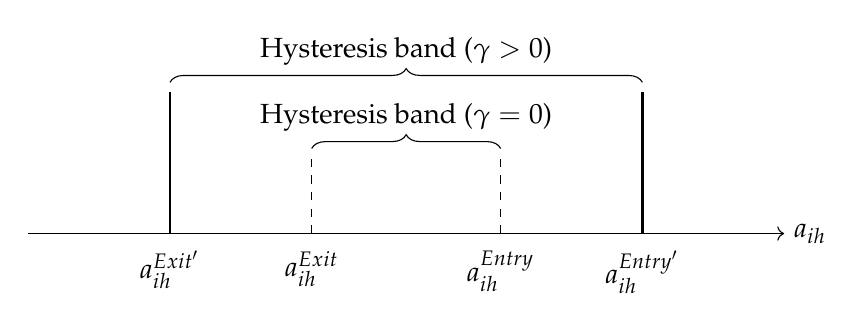
\begin{tikzpicture}[scale=1.2]

% Axis
\draw[->] (-4,0) -- (4,0) node[right] {$a_{ih}$};

% --- Baseline thresholds (gamma = 0) ---
\draw[dashed] (-1,0) -- (-1,0.8);
\node[below, yshift=-0.1cm] at (-1,0) {$a_{ih}^{Exit}$}; 

\draw[dashed] (1,0) -- (1,0.8);
\node[below, yshift=-0.1cm] at (1,0) {$a_{ih}^{Entry}$}; 

% --- Uncertainty thresholds (gamma > 0) ---
\draw[thick] (-2.5,0) -- (-2.5,1.5);
\node[below, yshift=-0.1cm] at (-2.5,0) {$a_{ih}^{Exit'}$}; 

\draw[thick] (2.5,0) -- (2.5,1.5);
\node[below, yshift=-0.1cm] at (2.5,0) {$a_{ih}^{Entry'}$}; 

% --- Braces above the axis ---
% For gamma = 0 (Lower brace, close to the axis)
\draw[decorate,decoration={brace,amplitude=5pt}]
(-1,0.9) -- (1,0.9)
node[midway,yshift=0.4cm] {Hysteresis band ($\gamma=0$)};

% For gamma > 0 (Upper brace)
\draw[decorate,decoration={brace,amplitude=5pt}]
(-2.5,1.6) -- (2.5,1.6)
node[midway,yshift=0.4cm] {Hysteresis band ($\gamma>0$)};

\end{tikzpicture}
\caption{Uncertainty widens the hysteresis band}\label{fig:band}
\end{figure}

\begin{description}
    \item[Hypothesis] \textit{The Brexit referendum reduces expected profitability and increases policy uncertainty. Under investment irreversibility arising from sunk entry and exit costs, uncertainty raises the option value of waiting and lowers the exit threshold for incumbent firms. As a result, affiliate exit responds substantially less than new entry.}
\end{description}



The combination of lower expected profitability and higher uncertainty expands the inaction region, thereby amplifying the asymmetry between entry and exit. A higher probability of deterioration ($\gamma > 0$) widens the hysteresis band by simultaneously raising the entry threshold and lowering the exit threshold. This asymmetric effect---driven by the interplay between sunk costs and policy uncertainty---predicts that the Brexit referendum reduced new Japanese FDI into the UK without triggering a proportional wave of affiliate exits.


Our model focuses on parent firm decision-making regarding foreign affiliate operations. In the following sections, we test these predictions using affiliate-level data because, while strategic decisions about market entry and exit ultimately originate with the parent firm, these decisions are implemented and manifested at the affiliate level, making affiliate-level data the most appropriate unit of analysis for testing our theoretical predictions.\footnote{At the same time, affiliate-level exit need not coincide with full withdrawal by the parent firm from the host country, especially when a parent operates multiple affiliates in the same market and can reorganize internally. To shed light on this margin, \ref{sec:multi_uk_affiliates} compares affiliate-level exit responses between parents with one UK affiliate and those with two or more UK affiliates in 2010.}




\section{Data and preliminary analysis \label{sec:data}}
\subsection{The Overseas Japanese Companies Data}

This study employs the frequently used Toyo Keizai Inc.'s Overseas Japanese Companies Data (hereafter, OJC data) (e.g., recently, among others, \citealt{Bederbos2021, cieslik2022brexit}). The OJC data contains basic information on Japanese parent firms' foreign affiliates. Importantly for this study, the OJC provides a detailed analysis of each affiliate's location.\footnote{See the following page for a more detailed description of the data: \url{https://biz.toyokeizai.net/en/data/service/detail/id=860}.} The OJC data is the best available data for the analysis of exits, as it is more complete than similar government databases with respect to the number of observations and foreign affiliate-specific information. 
For this study, we use OJC survey waves from 2010 to 2020. We harmonize the empirical panel to a two-year frequency throughout the analysis and use the 2010, 2012, 2014, 2016, 2018, and 2020 survey years. For each affiliate, the OJC provides the data of establishment, location, total capital, employment, and parent ownership information.\footnote{The capital is recorded in various currencies. It prevents us from using the capital data in our analysis.}


The OJC surveys provide the list of operating Japanese affiliates in each host country; affiliate exits are not specifically identified. Therefore, to determine an exit, we compare successive two-year survey observations to determine whether an affiliate is listed in both. When an affiliate is no longer listed in the OJC, it is considered having exited the host country.\footnote{For completeness, we ensure that there is not a survey error by examining subsequent OJC surveys to confirm exit.} Since the OJC survey takes place the year prior to its release (e.g., the OJC survey released in 1992 occurred in fall 1991), we use the year prior to the survey as the affiliate exit date.




\subsection{Preliminary analysis}

%%%%%%%%%%%%%%%%%%%%%%%%%%%%%%%%%%%%%%%%%%%%%%%%%%%%%%%%%%%%%%%%%%%

\begin{figure}[ht]
\begin{center}
    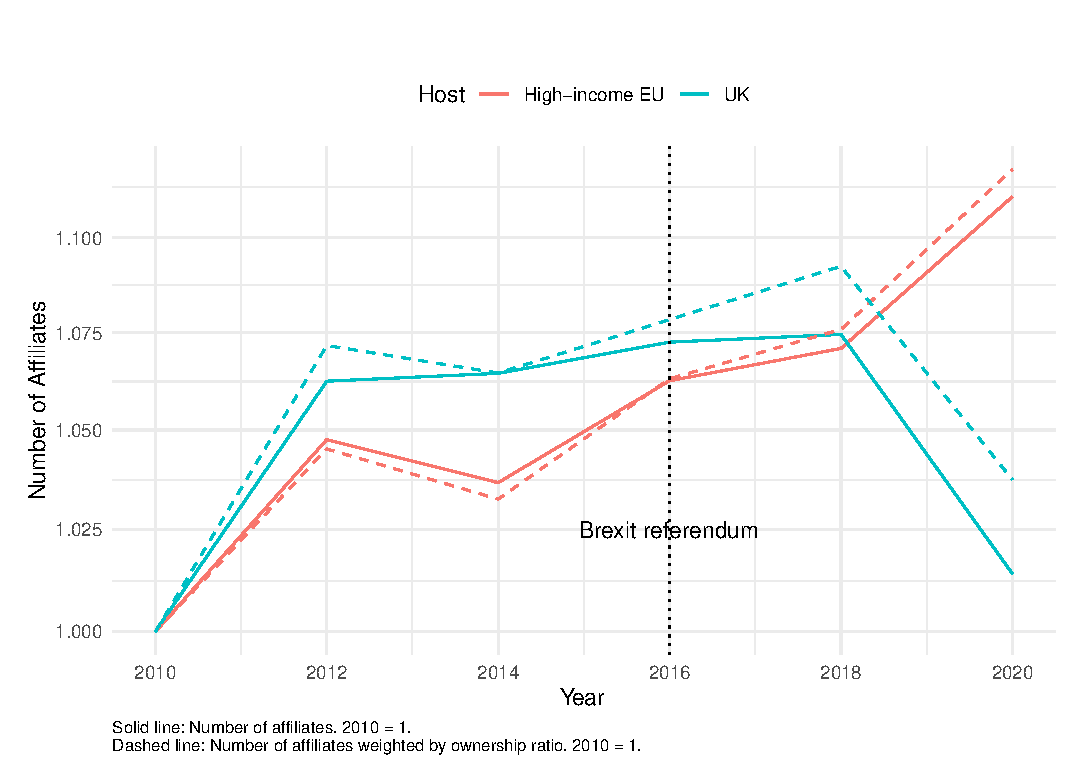
\includegraphics[keepaspectratio, scale=0.6]{Fig2.eps}
  
  \caption{Number of Japanese affiliates: UK and High-income EU}
    \label{fig:GBR_DEU}

\end{center}

\vspace{0.3cm}
\footnotesize
\emph{Source:} Authors' compilation based on Toyo Keizai's OJC data.

\emph{Notes:} Blue lines represents the values in the UK, while the red lines represents those in the comparison countries (High-income EU countries). The solid lines show the number of affiliates, while dashed lines show the number of affiliates weighted by Japanese ownership ratio. The values are normalized to set the 2010 value to one. 
\end{figure}
% Fig2_X2.Rmd
%%%%%%%%%%%%%%%%%%%%%%%%%%%%%%%%%%%%%%%%%%%%%%%%%%%%%%%%%%%%%%%%%%%

The OJC data provides us with several interesting insights into Japanese FDI in the UK. As Figure \ref{fig:GBR_DEU} indicates, there exists a leveling-off of the number of Japanese affiliates operating in the UK starting well before the Brexit referendum. Comparing the UK with other high-income EU countries (see Appendix Table \ref{tab:country-list} for the list of countries), in the UK, the number of affiliates dropped after the Brexit referendum. In contrast, in the other high-income EU countries, the number of affiliates continued to grow.
 
While informative, and supporting the notion that Japanese FDI fell in the post-referendum period, Figure \ref{fig:GBR_DEU} cannot tell us anything about why Japanese investment in the UK is lower.  We leave that to Figure \ref{fig:number}, which highlights Japanese exits and new entry into the UK.  Before the referendum, the number of new affiliates established in the UK approximately equaled UK exits, yielding the leveling-off of affiliate totals noted in Figure \ref{fig:GBR_DEU}. Exit and entry are much greater than in the other high-income EU countries, in part representing the large share of Japanese FDI that went into the UK relative to the rest of Europe. Importantly, note that after the decline in exits in 2016, exit from the UK quickly returned to previous levels.\footnote{This appears consistent with \cite{porto2023}, who find no short-run evidence of a decline in direct employment related to UK-based Japanese affiliates. In addition, they note the UK had experienced a declining share of European affiliates, especially between 2000--2010.} This is in contrast to new entries, which dropped for the UK to levels noted in the rest of the EU. By separating out exits and entries, it appears that the post-referendum decline in investment into the UK is not from increased exit, but rather from significantly decreased entry, although rigorous causal analysis is still required.

%%%%%%%%%%%%%%%%%%%%%%%%%%%%%%%%
\begin{figure}[ht]
\begin{center}
  \begin{minipage}[b]{0.45\linewidth}
    \centering
    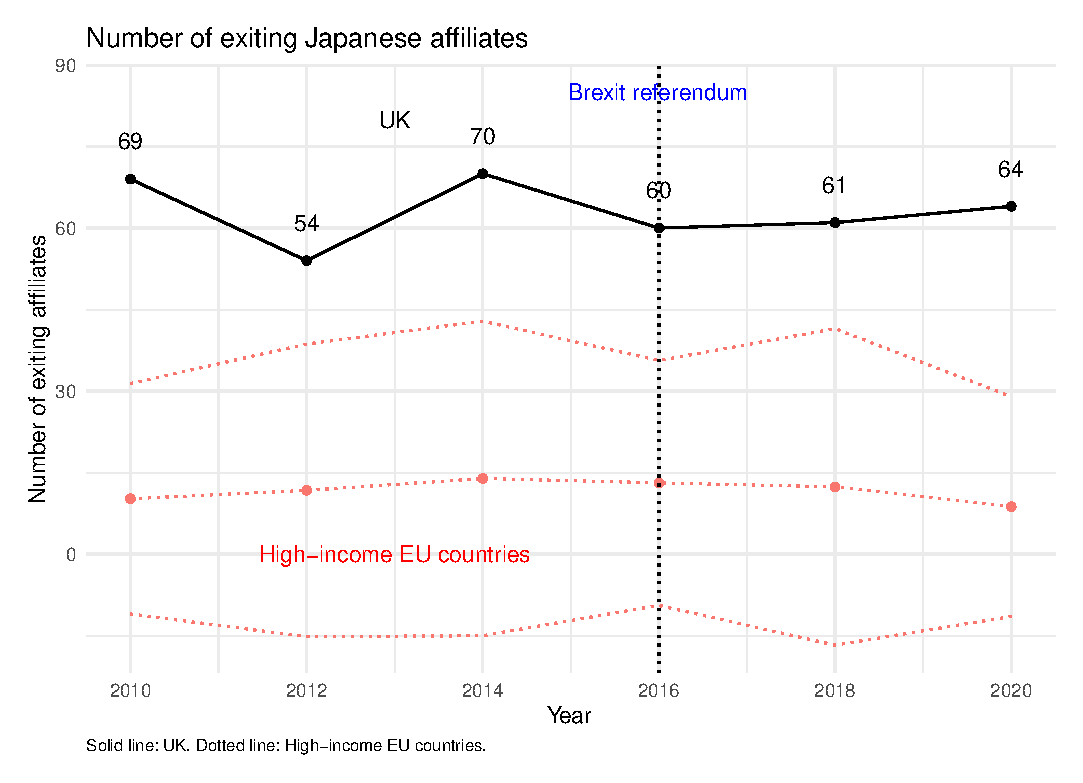
\includegraphics[keepaspectratio, scale=0.45]{Fig3a.eps}
    \subcaption{Number of exits}
  \end{minipage}
  \begin{minipage}[b]{0.45\linewidth}
    \centering
    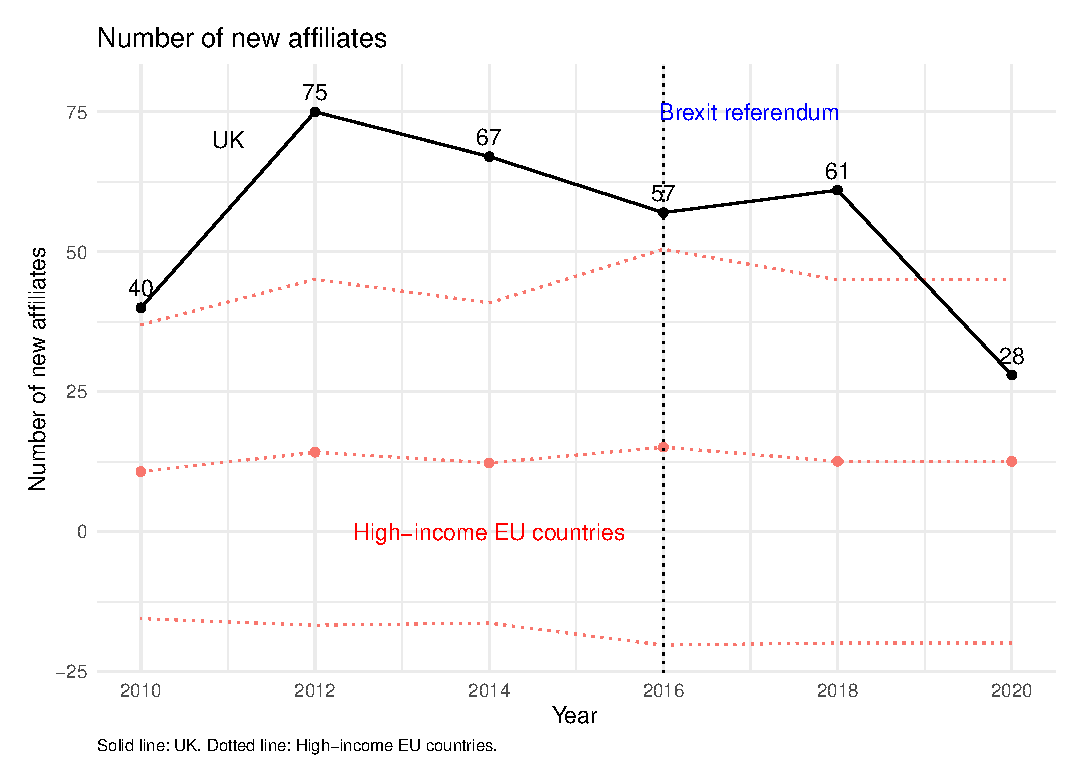
\includegraphics[keepaspectratio, scale=0.45]{Fig3b.eps}
    \subcaption{Number of new entries}
  \end{minipage}
  
  \caption{Number of Japanese affiliates}
    \label{fig:number}

\end{center}

\footnotesize
\emph{Source:} Authors' compilation based on Toyo Keizai's OJC data.\\
\emph{Note:} 
Panel (a) draws the number of Japanese affiliates exiting from a country, while Panel (b) draws those entering a country. The solid lines represent the numbers in the UK, while the dashed lines represent average numbers and confidence intervals in the other high-income EU countries.

\end{figure}
% A: Fig3a_X1_X3.Rmd
% B: Fig3b.Rmd
%%%%%%%%%%%%%%%%%%%%%%%%%%%%%%%%

\section{Empirical method \label{sec:method}}


\subsection{Two-way fixed effects (TWFE) model}

\subsubsection{Specification}

In order to identify the causal effects of the Brexit referendum on affiliate exit, we turn to the difference-in-differences method. We use a balanced panel of Japanese affiliates in the UK and other EU countries from 2010--2020, observed at two-year intervals: 2010, 2012, 2014, 2016, 2018, and 2020. We restrict our estimation sample to the affiliates that existed in the 2010 baseline wave, because affiliates that newly entered the UK especially after the referendum do not have comparable pre-treatment periods. In the baseline high-income EU sample, this restriction yields 1,694 affiliates and 10,164 affiliate-period observations. In the case of estimating the exit decision, we code the exit variable as 0 when an affiliate exists in the data and 1 after it finally disappears from the data. By doing so, we can examine whether the incumbent affiliates that existed in the UK before the referendum tended to experience an exit in the UK compared with those in other host countries.\footnote{In our online appendix, we provide simple Kaplan-Meier estimation to study Japanese exits from the UK. KM analysis enables us to assess the survival rates of different affiliate cohorts categorized by distinct characteristics (ie, affiliate location). Our results comparing UK and EU exits find the expected downward path dependence, indicating declining affiliate survival likelihood (or increased exit likelihood) as affiliates age. Importantly, results from a Mantel-Cox log-rank test indicate a p-value of 0.1, identifying no significant survival difference for Japanese affiliates in our two groups.}


Let $\mathcal{T}=\{2010,2012,2014,2016,2018,2020\}$ denote the set of survey years used in the empirical analysis.
We define the pre-referendum event-study years as $\mathcal{T}_{pre}=\{2010,2012\}$ and the post-referendum years as $\mathcal{T}_{post}=\{2016,2018,2020\}$, with 2014 omitted as the reference year.

Specifically, to investigate the time-varying effects of the referendum shock, we conduct a dynamic analysis using the following event study specification:
\begin{equation}\label{eq:es} 
% Callaway (2022), equation (9)
% Anderson, D. Mark, Kerwin Kofi Charles, Michael McKelligott, and Daniel I. Rees. 2022. "Estimating the Effects of Milk Inspections on Infant and Child Mortality, 1880−1910." AEA Papers and Proceedings 112: 188–92. https://doi.org/10.1257/pandp.20221066
Y_{i t}=\theta_{t}
+ \eta_{i}
+ \sum_{q \in \mathcal{T}_{pre}} \beta_{q} D_{i q}
+ \sum_{q \in \mathcal{T}_{post}} \beta_{q} D_{i q}
+v_{i t}
\end{equation}
where $i$ and $t \in \mathcal{T}$ index affiliate and survey year, respectively.
The outcome variable $Y_{it}$ is the indicator variable for an affiliate exit.
In the case of the exit model, the outcome variable, $Y_{it}$, is a binary variable that takes a value of zero if an affiliate $i$ exists in the data in period $t$ and is equal to 1 after the affiliate exits from the host country and disappear from the data.
The binary treatment variable, $D_{i t}$, is equal to 1 for affiliate $i$ in period $t$ if an affiliate $i$ is located in the UK in period $t$ and is equal to 0 otherwise. 
The coefficients, $\beta_{q}$, are expected to capture the treatment effects of the Brexit referendum.
As it is standard practice to choose the period prior to the event as the base period, we omit $t = 2014$ from equation (\ref{eq:es}), which normalizes the estimates of $\beta_{q}$ to 0 in that year.\footnote{See, for example, \cite{frey2021}.}
The equation (\ref{eq:es}) is often called two-way fixed effects (TWFE) model because it includes two-way fixed effects, that is affiliate fixed effects $\eta_{i}$ and year fixed effects $\theta_{t}$, in the estimation.\footnote{For the detailed description of the event study analysis and the TWFE model, see \cite{de2020two}, \cite{sun2021estimating}, \cite{callaway2023difference}, and \cite{roth2023survey} among others.}
The affiliate fixed effects absorb any time-invariant factors such as affiliate industry, affiliate type, and affiliate sizes.
Due to the high dimensional fixed effects, it becomes computationally difficult to use the logit or fractional logit models. We, therefore, use the standard alternative estimation technique (OLS) for our baseline exit analysis. In Section \ref{logit}, we complement these linear estimates with a pooled logit quasi-maximum likelihood estimator (QMLE) DiD specification following \citet{wooldridge2023simple}.

% Logistic Regression and the Incidental Parameters Problem
% https://gburtch.github.io/posts/2021/03/logit-ipp/

\subsubsection{Identifying assumptions}
To identify the causal effects of the Brexit referendum via equation (\ref{eq:es}), we need to assume the standard parallel trends assumption: 

\begin{align}\label{eq:pt}
\mathbb{E}\left[{Y_{i t}(0)}
-{Y_{i t^{\prime}}(0)} \mid \underbrace{D_{i}=1}_{\text{UK}} \right]
=
{\mathbb{E}\left[Y_{i t}(0)-Y_{i t^{\prime}}(0) \mid \underbrace{D_{i}=0}_{\text{Other EU}} \right]} 
\quad \textbf{for } t \neq t^{\prime} 
\end{align}
where $D_{i}$ is an indicator variable for the treated group, i.e., affiliate in the UK.\footnote{
See \cite{callaway2023difference} and \cite{roth2023survey} for a detailed explanation of the assumptions of the DiD method.
} 
Therefore, this assumption indicates that without the Brexit referendum, the average changes in the outcome of Japanese affiliates in the UK would be equal to those in other EU countries.

We also assume no anticipatory effects as follows:
\begin{align}
{Y_{i t}(0)}
=
Y_{i t}(1)  \text{ for } t \in \mathcal{T}, \; t < 2016 \text{ and for all } i \text { with } D_{i}=1.
\end{align}
This assumption states that the outcome before Brexit does not depend on the Brexit referendum. This assumption is validated by previous academic studies, and most of the popular press publications at the time, that indicated that a ``Leave" Brexit outcome was unlikely. For example, among others, \cite{becker_who_2017} discussed that bookmakers and pollsters predicted pre-Brexit that the ``Remain" side would win the referendum. \cite{alabrese_who_2019} also stated that the Brexit vote in the 2016 EU referendum came as a shock to many observers. We, therefore, consider the no anticipatory effects assumption is plausible.


Given the parallel trends assumption and no anticipatory effects assumption, the event study DiD specification (\ref{eq:es}) allows us to identify the average treatment effect on the treated (ATT):
\begin{align}
\tau _{2} = \mathbb{E} [ Y_{i2}(1) - Y_{i2}(0) | D_{i} = 1].
\end{align}
To validate the plausibility of the assumptions, we follow the standard practice of estimating the coefficients of the event study plot for the pre-treatment period.

\subsection{Extended two-way fixed effects model}\label{sec:etwfe_method}

The extended two-way fixed effects (ETWFE) model, proposed by \cite{wooldridge2021two}, is an extended version of the TWFE model that estimates post-treatment coefficients only and is robust to heterogeneous treatment effects.
The ETWFE model is specified as follows:
% Callaway (2023), equation (8)
\begin{align}\label{eq:ETWFE}
Y_{i t}=
\eta_{i}
+
\theta_{t}
+
\sum_{q \in \mathcal{T}_{post}}
\beta_{q}
\mathbf{1}\left\{D_{i}=1, t=q \right\}
+
v_{i t}
\end{align}
where $\eta_{i}$ and $\theta_{t}$ are affiliate and year fixed effects.
$D_{i}$ takes a value of one if an affiliate $i$ locates in the UK.
The calendar year, $q$, ranges over $\mathcal{T}_{post}$, namely, the post-treatment survey years.
The indicator variable, $\mathbf{1}\left\{D_{i}=1, t=q\right\}$, equals to one if an affiliate $i$ locates in the UK and year is $q$.
Therefore, $\mathbf{1}\left\{D_{i}=1, t=q\right\}$ indicates the post-treatment interaction terms.

The major difference between TWFE (\ref{eq:es}) and ETWFE (\ref{eq:ETWFE}) specifications is that ETWFE only estimates post-treatment coefficients.
In other words, the ETWFE model does not estimate pre-treatment coefficients.
Assuming that parallel trends hold in all pre-treatment periods, the ETWFE model omits to estimate parameters in pre-treatment periods and thus can produce more efficient estimates than the TWFE model if the assumption holds.
On the other hand, the TWFE event-study specification is often more informative about possible violations of parallel trends because it estimates pre-treatment lead coefficients explicitly.\footnote{See \cite{callaway2023difference} for more detailed discussion.}

\cite{wooldridge2021two} shows that, in the linear case, an ETWFE specification written with cohort indicators and cohort-by-time treatment interactions can be estimated using a pooled regression representation that is numerically equivalent to the formulation with the full set of unit fixed effects.\footnote{See \cite{wooldridge2021two}'s corollary 5.1 for a more precise statement.}
Therefore, instead of including the full set of affiliate fixed effects, $\eta_{i}$, we can use the pooled representation with treatment-group indicators and the relevant interaction terms while obtaining the same coefficient estimates for the dynamic treatment effects.
This greatly reduces the computational burden of the estimation.

\subsubsection*{Controls}

As \cite{wooldridge2021two} discussed, the ETWFE model allows the policy effects to change with time-constant controls $\mathbf{x}_{i}$.\footnote{See equation (5.15) of \cite{wooldridge2021two}.}
By using the controls, we can relax the parallel trends assumption so that the parallel trends assumption holds only conditional on the controls.
Under this conditional parallel trends assumption, the ETWFE model can identify the ATT.

Specifically, we extend the ETWFE model (\ref{eq:ETWFE}) by including the controls $\mathbf{x}_{i}$ as follows:
\begin{equation} \label{eq:ETWFE2} % Wooldridge (2021) (5.15)
\begin{array}{l}
Y_{i t}=
\eta_{i}
+
\theta_{t}
+
\sum_{q \in \mathcal{T}_{post}}
\beta_{q}
\mathbf{1}\left\{D_{i}=1, t=q\right\} \\
+
\sum_{q \in \mathcal{T}_{post}}
\mathbf{1}\left\{D_{i}=1, t=q\right\}
\cdot\left(\mathbf{x}_{i}-\boldsymbol{\mu}_{1}\right)
\boldsymbol{\gamma}_{q}
\\
+
\sum_{q \in \mathcal{T}_{post}}
\mathbf{1}\left\{t=q\right\}
\cdot \mathbf{x}_{i}
\boldsymbol{\delta}_{q}
+ v_{i t}
\end{array}
\end{equation}
where $\boldsymbol{\mu}_{1}$ is the average of controls among the treated affiliates, calculated as $\boldsymbol{\mu}_{1}=\overline{\mathbf{x}}_{1}=N_{1}^{-1} \sum_{i=1}^{N} D_{i} \cdot \mathbf{x}_{i}$.
For the exit analysis, we include affiliate employment and the number of affiliates in EU countries as controls. These covariates are chosen to capture observed differences in affiliate size and the firm's pre-existing exposure to the EU market that may be related to exit behavior.
Affiliate employment captures affiliate size, a key determinant of exit decisions, while the number of affiliates reflects network effects that may influence relocation and survival decisions, as noted by \citet{norback2015}.\footnote{\citet{norback2015} argue that the presence of other affiliates nearby can be positively correlated with divestiture.}
We use the baseline values of these controls measured in 2010.

\subsection{Nonlinear DiD}
\label{sec:method_entry}

Following \citet{wooldridge2023simple}, we use a common nonlinear DiD framework for both affiliate exit and new entry. In both cases, identification relies on the conditional no anticipation (CNA) and conditional index parallel trends (CIPT) assumptions. Let $g=2016$ denote the Brexit treatment cohort and let $\mathbf{x}$ collect time-invariant baseline covariates. CNA requires that treatment has no average effect before the referendum:
\begin{align}
E\!\left[Y_t(g)\mid D=1,\mathbf{x}\right] = E\!\left[Y_t(0)\mid D=1,\mathbf{x}\right], \qquad t<2016.
\end{align}
CIPT requires that, in the untreated state, the conditional mean can be written as
\begin{align}
E\!\left[Y_t(0)\mid D,\mathbf{x}\right] = G\!\left(\alpha + \delta D + m(\mathbf{x}) + r_t(\mathbf{x})\right),
\end{align}
where $G(\cdot)$ is a strictly increasing mean function and the trend component $r_t(\mathbf{x})$ does not vary with treatment status. The key identifying restriction is therefore that, conditional on $\mathbf{x}$, treatment assignment may affect levels of untreated outcomes but not their trend in the index. The two specifications below differ only in the choice of $G(\cdot)$ and the corresponding QMLE estimator.

\subsubsection{Pooled logit QMLE DiD for exit}

Because the exit outcome is binary, we choose the logistic mean function within this common framework. A convenient interpretation is given by the latent-index model
\begin{equation}
Y_{it}(0)=1\left[Y_{it}^{*}(0)>0\right],
\end{equation}
where $1[\cdot]$ is the indicator function and the latent variable satisfies
\begin{equation}
Y_{it}^{*}(0)=\alpha+\beta D_i+\gamma_t+U_{it},
\end{equation}
with $U_{it}$ continuous, independent of $D_i$, and identically distributed over time. Under this setup, CIPT implies a linear parallel trends restriction for the latent untreated outcome:
\begin{equation}
E\left[Y_{it}^{*}(0)\mid D_i\right]=\alpha+\beta D_i+\gamma_t.
\end{equation}
This is the binary-outcome analogue of Wooldridge's CNA/CIPT framework. In our context, it implies that, absent the Brexit referendum, the average evolution of the latent exit propensity for Japanese affiliates in the UK would have matched that of affiliates in the comparison countries.

For estimation, we follow \citet{wooldridge2023simple} and use a pooled logit quasi-maximum likelihood estimator (QMLE) DiD specification rather than a unit fixed-effects logit model. This choice is motivated by two practical considerations. First, logit models with high-dimensional affiliate fixed effects are computationally difficult and, in our data, failed to converge. Second, fixed-effects estimators in nonlinear panel models are subject to the incidental parameters problem \citep{fernandez2009fixed, fernandez2018fixed}. The pooled logit QMLE DiD specification avoids these issues by using a pooled representation with group-level treatment timing rather than a full set of affiliate fixed effects, while still delivering ATT estimates that are directly comparable to our linear DiD results.

As in the linear case, we assume no anticipatory effects before 2016. Following \citet{wooldridge2023simple}, we assess the plausibility of CNA and CIPT by examining the pre-treatment coefficients from the pooled nonlinear DiD specification. With the canonical logit link and the corresponding pooled QMLE event-study specification, this test is numerically equivalent to testing the relevant restrictions using untreated observations only. In our application, the cluster-robust Wald test cannot reject the null that the pre-treatment coefficients are jointly zero (p-value $= 0.995$), which supports the plausibility of the nonlinear identifying assumptions.

\subsubsection{Pooled Poisson QMLE DiD for entry}

To fully test the asymmetric impact of Brexit-related uncertainty predicted by our theoretical framework, we extend our analysis to the extensive margin of new affiliate entries. While the exit analysis focuses on incumbent firms anchored by sunk costs, the entry analysis examines whether the post-referendum environment deterred potential investors who had not yet committed to those costs.

Given that new entries are represented as non-negative counts, we aggregate the number of new Japanese affiliate entries at the host country-industry-survey-year level.
Following \citet{wooldridge2023simple}, we employ the pooled Poisson QMLE. The use of Poisson QMLE is well established in the trade literature, and its application in the context of DiD and event-study analyses has recently been demonstrated by \cite{nagengast2025staggered} and \cite{nagengast2026european}.
The empirical specification for the entry analysis is:

\begin{equation}\label{eq:entry_ppml}
Y_{hkt} = \exp\left( \alpha + \delta D_h + \lambda_{kt} + \sum_{\tau \in \mathcal{T}_{pre} \cup \mathcal{T}_{post}} \beta_{\tau} (D_h \times \mathbb{1}[t=\tau]) + \mathbf{x}_{hk}\boldsymbol{\gamma} \right) + \epsilon_{hkt}
\end{equation}
where $Y_{hkt}$ is the count of new Japanese affiliate entries in host country $h$ and industry $k$ in survey year $t \in \mathcal{T}$. As emphasized by \citet{wooldridge2023simple}, including a full set of unit fixed effects in nonlinear models makes the computation of ATTs and their valid standard errors notably difficult. Therefore, instead of using country fixed effects, we include a constant $\alpha$ and a cohort dummy $D_h$ to indicate the treated country. $\lambda_{kt}$ denotes survey-year-by-industry dummy variables, which absorb common industry-specific time trends and global industry-level shocks. The vector $\mathbf{x}_{hk}$ includes time-invariant, industry-level baseline controls measured at 2010, specifically the median affiliate size in each host country-industry cell, which captures pre-existing differences in the scale of Japanese investment activity across sectors and adjusts for baseline outcome levels.

The coefficients of interest, $\beta_{\tau}$, capture the dynamic impact of the Brexit referendum on new entries relative to the reference year (2014). Following our hypothesis in Section \ref{sec:Model}, we expect $\beta_{\tau}$ to be significantly negative for $\tau \geq 2016$, reflecting the increased entry threshold ($a^{Entry}$) due to heightened policy uncertainty.

Equation \eqref{eq:entry_ppml} is estimated via pooled Poisson QMLE using all observations. 
The pooled Poisson QMLE belongs to the linear exponential family (LEF) and its key robustness property is that consistency of $\hat{\beta}_{\tau}$ requires only correct specification of the conditional mean $E[Y_{hkt}|\cdot] = \exp(\cdot)$; no restrictions are imposed on higher moments of $\epsilon_{hkt}$, including serial correlation across periods and overdispersion \citep{wooldridge2023simple}.
For nonnegative count outcomes, the exponential mean combined with the Poisson quasi-log likelihood constitutes the canonical link function pairing in the LEF \citep[Table 1]{wooldridge2023simple}, which guarantees that the pooled QMLE and the imputation estimator yield numerically identical estimates of $\beta_{\tau}$ and their standard errors.
As noted by \citet{wooldridge2023simple}, Poisson models are also a special case in which including unit fixed effects does not generate the incidental parameters problem for coefficient estimation. However, obtaining ATT estimates on the original outcome scale and valid standard errors is considerably more straightforward in the pooled Poisson QMLE DiD framework. We therefore adopt the latter in our entry analysis.
Furthermore, \citet{wooldridge2023simple} shows that the identifying assumptions can be stated conditional on time-invariant covariates. In our setting, the baseline controls in $\mathbf{x}_{hk}$ play that role, while the survey-year-by-industry dummy variables $\lambda_{kt}$ absorb common industry-specific shocks and secular trends that are shared across host countries within each industry. The assumptions in this subsection are the entry-specific specialization of Wooldridge's CNA/CIPT framework.

In our setting, CNA requires that the Brexit referendum exerted no effect on new affiliate entries prior to 2016:
\begin{align}
E[Y_{hkt}(g) \mid D_h, \mathbf{x}_{hk}] = E[Y_{hkt}(0) \mid D_h, \mathbf{x}_{hk}], \quad t < g,
\end{align}
where $Y_{hkt}(0)$ is the potential entry count in the never-treated state and $Y_{hkt}(g)$ denotes the potential outcome path associated with treatment cohort $g$. In our application, the only treated cohort is $g=2016$. 

For the exponential mean specification, CIPT states that the conditional mean of the untreated potential outcome takes the form:
\begin{align}\label{eq:cipts}
E[Y_{hkt}(0) \mid D_h, \mathbf{x}_{hk}] = \exp\!\left(\alpha + \delta D_h + \lambda_{kt} + \mathbf{x}_{hk}\boldsymbol{\gamma}\right).
\end{align}
The key restriction embedded in \eqref{eq:cipts} is that the time trend $\lambda_{kt}$ does not interact with $D_h$: conditional on industry and the baseline covariate $\mathbf{x}_{hk}$, the growth rate of potential entry counts evolves proportionally for the UK and comparison countries.
Equivalently, CIPT implies the following ratio-form parallel trends condition:
\begin{align}\label{eq:pt_ratio}
\frac{E[Y_{hkt}(0) \mid D_h=1,\, \mathbf{x}_{hk}]}{E[Y_{hkt'}(0) \mid D_h=1,\, \mathbf{x}_{hk}]}
=
\frac{E[Y_{hkt}(0) \mid D_h=0,\, \mathbf{x}_{hk}]}{E[Y_{hkt'}(0) \mid D_h=0,\, \mathbf{x}_{hk}]}, \quad t \neq t'.
\end{align}
This ratio condition is considerably more plausible for count outcomes than the standard linear parallel trends assumption, as it requires only proportional---rather than level---comovements in the untreated conditional mean \citep{wooldridge2023simple}. In our empirical implementation, the survey-year-by-industry dummy variables $\lambda_{kt}$ flexibly absorb industry-specific aggregate shocks and common secular trends. This does not by itself guarantee CIPT, but it makes the assumption more plausible within industry by allowing untreated trends to differ systematically across industries. Unlike standard TWFE models with unit fixed effects, the pooled Poisson QMLE approach identifies the proportionate change in entry counts attributable to Brexit through cohort and event-time interactions under CNA and CIPT.
We cannot directly test the CIPT and CNA assumptions, but we can examine the pre-treatment event study coefficients $\beta_{2010}$ and $\beta_{2012}$ in equation \eqref{eq:entry_ppml} to assess whether there were any significant differences in entry trends between the UK and comparison countries prior to Brexit. If these coefficients are not statistically significant, it would provide supportive evidence for the validity of the parallel trends assumption underlying our identification strategy.
As a robustness check for potential pre-treatment trend violations observed in the early 2010s, we also use the synthetic DiD method to ensure the results are robust.

\subsection{Synthetic DiD}

While TWFE relies on the parallel trends assumption holding exactly, SDiD reduces reliance on this assumption by reweighting control units to better match pre-treatment outcome paths, thereby providing more credible estimates even when pre-treatment trends are not perfectly parallel. As an additional robustness check, we employ the SDiD estimator proposed by \citet{arkhangelsky2021synthetic}, which combines the main advantages of DiD and synthetic control and remains applicable in panel settings with many units, allowing conventional inferential procedures.
Unlike the standard TWFE estimator, SDiD assigns weights $\hat{\omega}_{i}$ to control units so that their pre-treatment trends more closely match those of the treated units, and weights $\hat{\lambda}_{t}$ to pre-treatment periods that are more representative of the post-treatment period, thereby making the parallel trends assumption more plausible.

In SDiD, we include unit fixed effects ($\eta_{i}$) and year fixed effects ($\theta_{t}$), as in a standard two-way fixed effects regression. In addition, SDiD introduces two sets of weights. The unit weights ($\hat{\omega}_{i}$) are chosen so that the pre-treatment trend in the weighted control group is as parallel as possible to that of the treated group, rather than requiring exact matching as in the standard synthetic control method. The time weights ($\hat{\lambda}_{t}$) balance pre-treatment periods against post-treatment periods.\footnote{
The unit weights $\hat{\omega}_{i}$ are chosen to minimise the discrepancy between the weighted control pre-treatment trends and the treated pre-treatment trends, with an intercept that permits parallel rather than exact matching and an $L_{2}$ regularisation penalty to prevent the weights from concentrating on a single unit (equation 4 of \citealt{arkhangelsky2021synthetic}).
The time weights $\hat{\lambda}_{t}$ are chosen so that the weighted average of pre-treatment periods is as representative as possible of the post-treatment period, with an intercept allowing a constant shift between the two (equation 6 of \citealt{arkhangelsky2021synthetic}).
}
Using these two weights, SDiD estimates the average effect of the Brexit referendum by minimizing the weighted residual sum of squares:
\begin{align} \label{eq:SDiD}
\left(\hat{\tau}, \hat{\mu}, \hat{\eta}, \hat{\theta}\right)
=
\underset{\tau, \mu, \eta, \theta}{\arg \min }
\left\{\sum_{i=1}^{N} \sum_{t \in \mathcal{T}}
\left(Y_{i t}-\mu-\eta_{i}-\theta_{t}
-D_{i t} \tau \right)^{2}
\underbrace{\hat{\omega}_{i} \hat{\lambda}_{t}}_{\text{weights}}
\right\}
\end{align}
where $N$ is the number of units and $\mathcal{T}$ is the set of survey years. $Y_{it}$ is the outcome variable and $\mu$ is the constant.
The Brexit dummy, $D_{it}$, takes a value of one if the host country is the UK and $t \geq 2016$ and zero otherwise.

We apply this SDiD framework to both exit and entry analyses.
The interpretation of the unit fixed effects $\eta_{i}$ and unit weights $\hat{\omega}_{i}$ differs across the two applications.
In the exit analysis, the unit of observation is an individual affiliate, so $\eta_{i}$ denotes affiliate fixed effects and $\hat{\omega}_{i}$ are affiliate-level weights; the outcome $Y_{it}$ is the binary exit indicator.
In the entry analysis, the unit of observation is a host country-industry cell, so $i$ indexes country-industry pairs, $\eta_{i}$ denotes host country-industry fixed effects and $\hat{\omega}_{i}$ are country-industry-level weights; the outcome $Y_{it}$ is the count of new Japanese affiliate entries.
In both cases, the treatment indicator $D_{it}$ equals one if the host country is the UK and $t \geq 2016$, and zero otherwise.


\section{Aggregate entry-exit benchmark}\label{sec:aggregate_benchmark}

Before turning to the more detailed affiliate-level analyses of exit and entry, we first present an aggregate benchmark that places both in a common empirical framework. Table \ref{tab:2x2did_aggregate} reports a simple $2\times2$ DiD model estimated by Poisson Pseudo Maximum Likelihood (PPML) for the two-year survey waves from 2010 to 2020, using country-industry-survey-year outcomes. The dependent variables are the total number of Japanese affiliates, the number of exits, and the number of new entries, respectively.

This table is useful for evaluating the entry-exit asymmetry because all three outcomes are measured at the same country-industry-survey-year level, use the same treated unit, post-referendum indicator, comparison countries, and PPML functional form. The coefficient on $UK \times \text{Post-Referendum}$ is negative and highly significant for new affiliate entry, whereas the corresponding coefficients for the total number of affiliates and exits are small and statistically insignificant. To assess the difference formally, we also estimate a stacked PPML model with margin-by-treatment interactions and test equality of the absolute magnitudes of the entry and exit DiD coefficients. The estimated difference in absolute values, $\left|\textrm{New Entry DiD}\right|-\left|\textrm{Exit DiD}\right|$, is positive and statistically significant ($0.294$, s.e. $0.118$). Thus, in a common aggregate framework, the referendum-period change is concentrated on the entry margin rather than on the exit margin.

We do not interpret Table \ref{tab:2x2did_aggregate} as the final evidence on either margin, because entry and exit remain distinct outcomes and the detailed analyses below use richer outcome-specific information. Instead, the table provides a transparent benchmark showing that the asymmetric pattern is not generated only by comparing unrelated specifications. The next section examines the exit margin using affiliate-level DiD, nonlinear DiD, and synthetic DiD estimators, while Section~\ref{sec:entry} analyzes new entry in greater detail.


%%%%%%%%%%%%%%%%%%%%%%%%%%%%%%%%
{\renewcommand\normalsize{\scriptsize}%
\normalsize 
\begin{table}[!ht]
\centering
\caption{\label{tab:export-latex}Impact of Brexit Referendum on Japanese FDI (2x2 DiD)\label{tab:2x2did_aggregate}}
\centering
\begin{threeparttable}
\begin{tabular}[t]{lccc}
\toprule
  & Total Affiliates & Exits & New Entry\\
\midrule
UK & 1.532*** & 1.684*** & 1.588***\\
 & (0.383) & (0.326) & (0.347)\\
Post-Referendum & 0.051 & -0.047 & 0.078\\
 & (0.033) & (0.073) & \vphantom{1} (0.085)\\
UK x Post-Referendum & -0.040 & 0.004 & -0.298***\\
 & (0.033) & (0.073) & (0.085)\\
\midrule
Num.Obs. & 5040 & 5040 & 5040\\
$\left|\textrm{New Entry DiD}\right| - \left|\textrm{Exit DiD}\right|$ &  &  & 0.294*\\
 &  &  & (0.118)\\
Equality test p-value &  &  & 0.013\\
Pseudo R-squared & 0.091 & 0.082 & 0.055\\
\bottomrule
\end{tabular}

\end{threeparttable}\par\medskip
\parbox{\linewidth}{\footnotesize Notes: Standard errors clustered by host country are reported in parentheses. The estimates use country-industry-survey-year outcomes. The dependent variables are the total number of Japanese affiliates, the number of exits, and the number of new entries, respectively. All models are estimated using Poisson Pseudo Maximum Likelihood (PPML). The row $\left|\textrm{New Entry DiD}\right| - \left|\textrm{Exit DiD}\right|$ reports the difference in absolute values of the new-entry and exit DiD coefficients, computed via the delta method from a stacked PPML model with margin-by-treatment interactions (assuming opposite signs: exit DiD $>$ 0, entry DiD $<$ 0); its p-value tests equality of the absolute magnitudes. The comparison group consists of 11 high-income EU countries (AUT, BEL, DNK, FIN, FRA, DEU, IRL, ITA, LUX, NLD, SWE). * p $<$ 0.05, ** p $<$ 0.01, *** p $<$ 0.001.
}

\end{table}

}
% Tab1.Rmd
%%%%%%%%%%%%%%%%%%%%%%%%%%%%%%%%

\section{Affiliate exit responses \label{sec:results}}
\subsection{Baseline results}\label{sec:twfe}

We conduct a dynamic analysis using the event study specification in equation (\ref{eq:es}) to estimate the time-varying effects of the Brexit referendum on affiliate exits in the UK during the 2016--2020 uncertainty period. 
The event study coefficients are presented in Figure \ref{fig:es1} with the 95\% confidence intervals.
Figure \ref{fig:es1} presents the effects of the Brexit referendum on affiliates' exit probability.
The figure uses affiliates in the UK as the treated group.
High-income EU countries serve as the comparison countries. They are Luxembourg, Ireland, Denmark, Netherlands, Sweden, Austria, Germany, Finland, Belgium, France, and Italy.
We consider the high-income EU countries to be a more suitable comparison group than lower-income EU countries because the former tend to be more similar to the UK from the viewpoint of Japanese investors. The list of high-income EU countries is provided in the Appendix Table \ref{tab:country-list}.


%%%%%%%%%%%%%%%%%%%%%%%%%%%%%%%%%%%%%%%%%%%%%%%%%%%%%%%%
\begin{figure}[ht]
\begin{center}

    \includegraphics[keepaspectratio, scale=0.6]{Fig4.eps}

 \caption{Dynamic impacts of the Brexit referendum on exit probability}
    \label{fig:es1}
    
\end{center}

\footnotesize
\emph{Source:} Authors' compilation based on Toyo Keizai's OJC data.\\
\emph{Note:} The figures present the event study coefficients of equation (\ref{eq:es}) with the 95\% confidence intervals. 
The value labels indicate the estimates of the coefficients when we use the high-income EU countries as the comparison countries.
The figure draws the affiliate-level effects of the Brexit referendum on the exit probability.
The R \texttt{fixest} package \citep{fixest} is used.

\end{figure}
% Tab2_Fig4.Rmd
%%%%%%%%%%%%%%%%%%%%%%%%%%%%%%%%%%%%%%%%%%%%%%%%%%%%%%%%

Figure \ref{fig:es1} shows the effects of the Brexit referendum on the affiliate exit probability.
The coefficient estimates of the event study plots on the exit probability in Figure \ref{fig:es1} are relatively small, ranging from 0.9 percentage points in 2016 to 2.9 percentage points in 2020 on average. 
Furthermore, they are not statistically significant at the 5\% level.
There is a slightly upward trend in Figure \ref{fig:es1}, especially between the 2018 and 2020 survey waves.
However, we do not find any significant evidence that the Brexit referendum pushed Japanese affiliates out of the UK during the period we study.


%we have to note that the UK faced severe pandemic impacts in those years.

We also note that the pre-treatment coefficients are not significant, suggesting that the parallel trends assumption holds.
This implies that the estimated referendum-period effects on affiliate exits are not biased by the pre-treatment differences between the UK and other high-income EU member countries.

To summarize, our baseline event study analysis indicates that the Brexit referendum had a negligible effect on the exit probability of Japanese multinationals in the UK during the referendum-to-exit period, consistent with our model’s prediction that hysteresis effects discourage exit.
As an additional heterogeneity exercise, \ref{sec:parent_uk_exposure} reports affiliate-level event-study estimates split by the parent firm's pre-referendum UK exposure and shows that the estimated exit response is larger among affiliates whose parent firms were more exposed to the UK before the referendum.





%\subsection{Robustness checks}\label{sec:robustness}

\subsection{Extended two-way fixed effects model}\label{sec:etwfe}

As described in Section~\ref{sec:etwfe_method}, we employ the ETWFE model of \cite{wooldridge2021two} as a robustness check to estimate the post-treatment effects of the Brexit referendum on affiliate exits in the UK.
The following table shows the estimation result of the ETWFE model.\footnote{We used \cite{etwfe}'s R package \texttt{etwfe}.} 
Columns (1) and (2) present the results for exit probability.
Column (1) uses high-income EU member countries as comparison countries, while Column (2) uses all other EU member countries as comparison countries.
The table shows estimated coefficients of the post-treatment interaction terms for the three post-referendum survey years, 2016, 2018, and 2020.
The estimated coefficients of the ETWFE model are quite similar to those of the TWFE model in the previous section.
The post-treatment interaction terms are not significant in either specification at the conventional levels, indicating that the referendum-period effects on the exit probability are not significant regardless of comparison countries. 
In sum, the results from the ETWFE model are consistent with those from the TWFE model, indicating that, as our model predicts, the effects of the Brexit referendum on affiliate exits in the UK are negligible.


%%%%%%%%%%%%%%%%%%%%%%%%%%%%%%%%
{\renewcommand\normalsize{\scriptsize}%
\normalsize 
\begin{table}[!ht]
\centering
\caption{\label{tab:Table-ETWFE-OLS}Effect of the Brexit Referendum on Exit Probability (ETWFE, OLS)}
\centering
\begin{tabular}[t]{lcc}
\toprule
\multicolumn{1}{c}{ } & \multicolumn{2}{c}{Exit probability} \\
\cmidrule(l{3pt}r{3pt}){2-3}
 & (1) & (2)\\
\midrule
UK $\times$ 2016 & 0.011 & 0.007\\
 & (0.026) & (0.023)\\
UK $\times$ 2018 & 0.007 & 0.004\\
 & (0.028) & (0.025)\\
UK $\times$ 2020 & 0.032 & 0.027\\
 & (0.032) & (0.028)\\
Num.Obs. & 10164 & 11568\\
Group Fixed-Effects & Yes & Yes\\
Two-year Period Fixed-Effects & Yes & Yes\\
R2 & 0.104 & 0.104\\
\bottomrule
\end{tabular}
\begin{flushleft}
\footnotesize
Notes: Marginal effects from Wooldridge's (2021) extended two-way fixed effects (ETWFE) model are reported in the table. Standard errors are clustered at the country level and presented in parentheses. The data are affiliate-level balanced panel data from the OJC data. The estimation uses data from 2010 to 2020, with event-time indicators grouped into two-year bins and the 2014--2015 bin omitted as the reference period. To improve computational efficiency, the estimation employs group-level (i.e., country-level) fixed effects instead of unit-level (i.e., affiliate-level) fixed effects. This estimation strategy follows Wooldridge (2021), which demonstrates the equivalence of group- and unit-level fixed effects in linear models. The R package `etwfe` is used for implementation. * $p<0.05$, ** $p<0.01$, *** $p<0.001$.
\end{flushleft}
\end{table}

}
% Tab2_Fig4.Rmd
%%%%%%%%%%%%%%%%%%%%%%%%%%%%%%%%





\subsubsection*{Controls with imputation}

When using employment data from foreign affiliates, we encountered missing values that required imputation.
We employed three approaches to handling missing affiliate employment. The first is the \textit{mean imputation method}, which replaces missing values of affiliate employment with the country-survey-year average.
The second is the \textit{multiple imputation method}, implemented via Predictive Mean Matching (PMM) using the \texttt{mice} package in R.\footnote{\cite{hayati2015rise} describe the multiple imputation method.}
The third is a \textit{complete-case analysis}, which drops observations with missing affiliate employment.

Our multiple imputation procedure generated five imputed datasets ($m=5$), based on a predefined predictor matrix that included the number of Japanese parent firms, the number of affiliates in Europe, and the number of years since establishment. To ensure convergence, we ran 50 iterations of the algorithm.
The PMM procedure consists of several steps. First, we fit regression models for affiliate employment using the specified predictors. At each iteration, we draw parameter values from their posterior distributions and calculate predicted values for both complete and incomplete cases.  
For each missing observation, we identify a set of donor cases with predicted values closest to that of the incomplete case and randomly select one donor to impute the missing value using its observed outcome.  
This process is repeated across all 50 iterations, resulting in five completed datasets that reflect both parameter uncertainty and residual variability.  


Using the imputed data, we estimated the effect of the Brexit referendum using the ETWFE model (\ref{eq:ETWFE2}) with controls.
For multiple imputation, we fitted the ETWFE model to each of the five imputed datasets, generating five separate estimates. These estimates were then combined using Rubin’s rules, which account for both within-imputation and between-imputation variance, to produce a single, robust estimate per event time.



Figure~\ref{fig:imputed} presents event study plots based on these three approaches. The figure compares mean imputation, multiple imputation, and complete-case analysis. The plots indicate that the estimated effect of the Brexit referendum on exit probability is statistically insignificant at conventional levels regardless of how missing affiliate employment is handled. These findings are consistent in both magnitude and statistical significance with those reported in the ETWFE table above and Figure~\ref{fig:es1}, and further support our prediction that hysteresis discourages exit. The sample sizes differ across the three series for mechanical reasons. Mean imputation uses the full sample because all missing employment values are replaced by country-survey-year averages. Multiple imputation retains almost the full sample, but a small number of observations remain unavailable after the PMM procedure, which is why the reported $N$ is slightly smaller. By contrast, the complete-case estimates use only observations with non-missing employment in the raw data and therefore rely on a considerably smaller sample.



%%%%%%%%%%%%%%%%%%%%%%%%%%%%%%%%%%%%%%%%%%%%%%%%%%%%%%%%%
\begin{figure}[ht]
  \begin{center}
    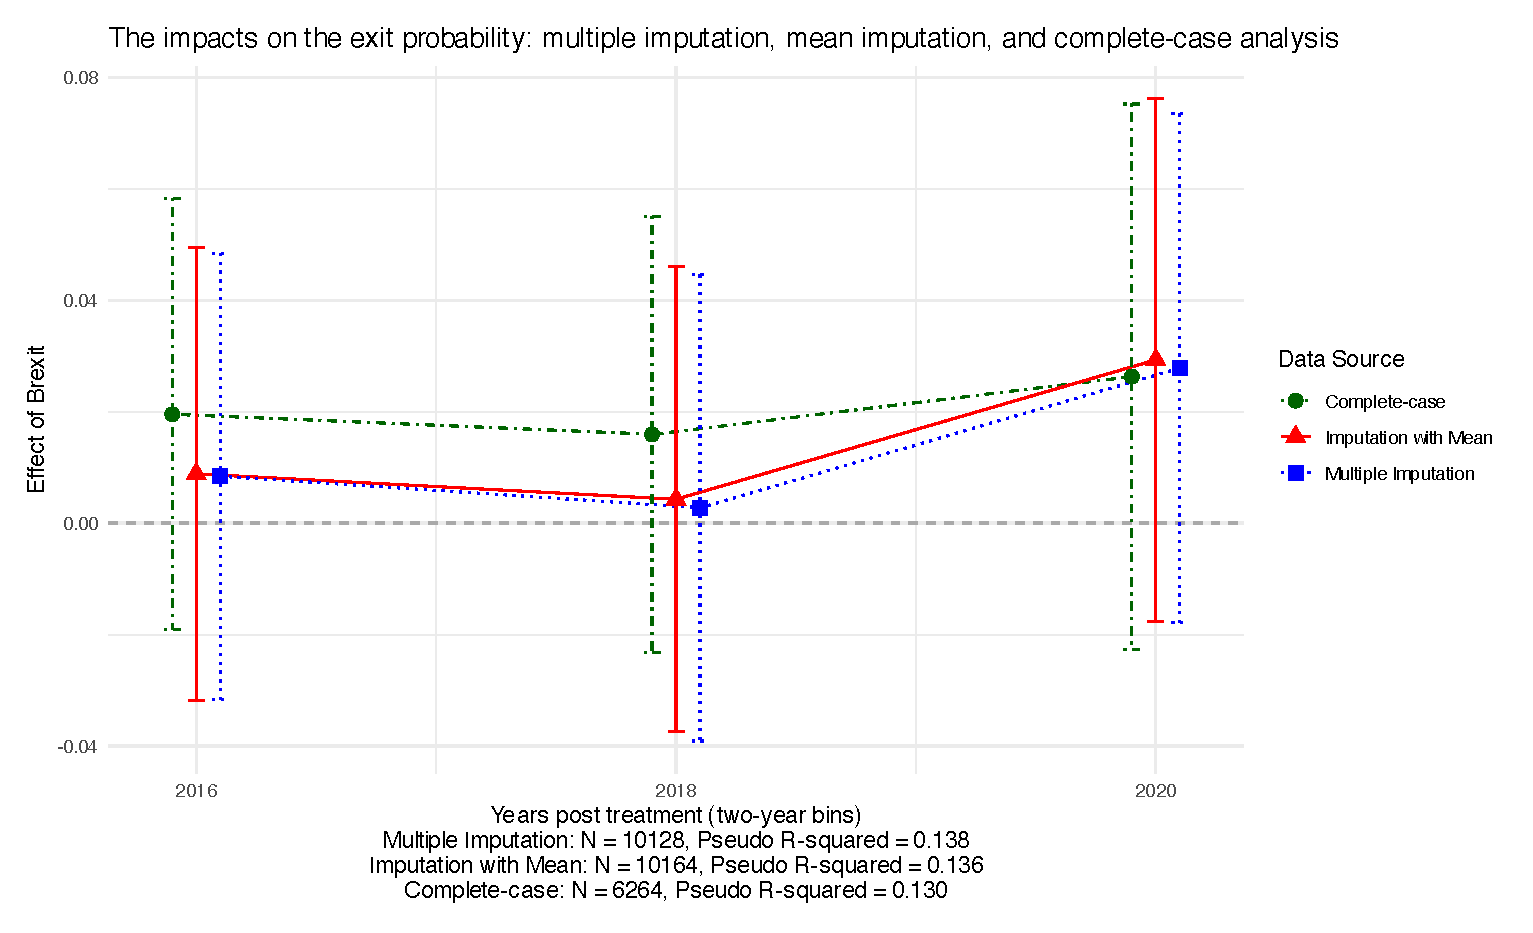
\includegraphics[width=0.8\linewidth]{Fig5.eps}
    \caption{The Brexit referendum's impact on exit probability under alternative treatments of missing employment data}
    \label{fig:imputed}

  \end{center}

    \footnotesize
    \emph{Source:} Authors' compilation based on Toyo Keizai's OJC data.\\
    \emph{Note:} The figures present the event study coefficients of equation (\ref{eq:ETWFE2}) with the 95\% confidence intervals. 
    The figure draws the affiliate-level effects of the Brexit referendum on the exit probability.
    The three lines correspond to mean imputation, multiple imputation, and complete-case analysis.
    We use the high-income EU countries as the comparison countries.
    The R \texttt{etwfe} package is used.
\end{figure}
% Fig5.Rmd
%%%%%%%%%%%%%%%%%%%%%%%%%%%%%%%%%%%%%%%%%%%%%%%%%%%%%%%%%



\subsection{Pooled Logit QMLE DiD for Exit}\label{logit}

So far, we have used linear DiD models to estimate the effects of the Brexit referendum on the exit probability of Japanese affiliates in the UK. As discussed in Section \ref{sec:method}, we now compare those linear estimates with the pooled logit QMLE DiD specification of \citet{wooldridge2023simple} for a binary outcome. This provides a nonlinear robustness check that is well suited to affiliate exit and avoids the computational and incidental-parameters problems associated with fixed-effects logit estimation.

The estimation results of the logit model are presented in Figure \ref{fig:logit}. 
The figure shows the event-study coefficients from the pooled logit QMLE DiD specification with the 95\% confidence intervals.
Basically, the results of the logit model are consistent with those of the OLS model.
The estimated effects of the Brexit referendum on the exit probability are not significant at the conventional levels.
Furthermore, the estimated ATTs are close to those of the baseline model and the linear ETWFE specification. 
The results suggest that the effects of the Brexit referendum on affiliate exits are limited and negligible regardless of the model specification. 

%%%%%%%%%%%%%%%%%%%%%%%%%%%%%%%%%%%%%%%%%%%%%%%%%%%%%%%%
\begin{figure}[ht]
\begin{center}

    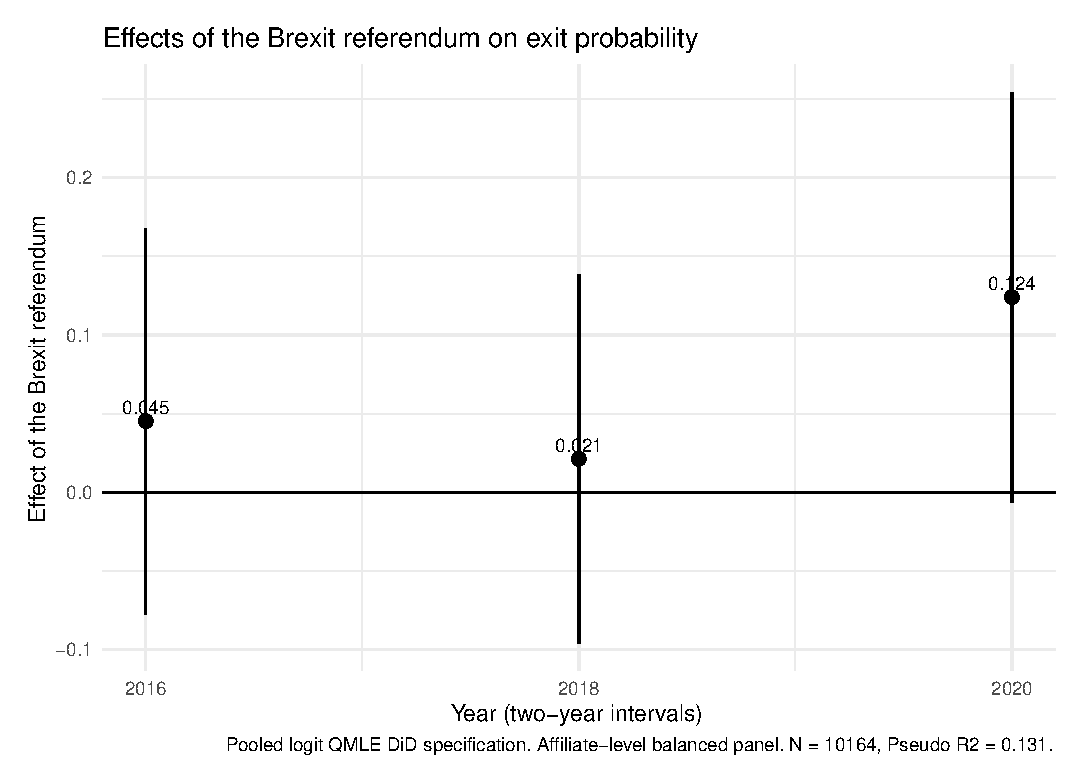
\includegraphics[keepaspectratio, scale=0.6]{Fig6.eps}

 \caption{Dynamic impacts of the Brexit referendum on exit probability (Nonlinear DiD)}
    \label{fig:logit}
    
\end{center}

\footnotesize
\emph{Source:} Authors' compilation based on Toyo Keizai's OJC data.\\
\emph{Note:} The figures present the event-study coefficients of the pooled logit QMLE DiD specification following \cite{wooldridge2023simple}, with the 95\% confidence intervals. 
The figure draws the affiliate-level effects of the Brexit referendum on the exit probability.
The R \texttt{etwfe} package is used.

\end{figure}
% Fig6.Rmd
%%%%%%%%%%%%%%%%%%%%%%%%%%%%%%%%%%%%%%%%%%%%%%%%%%%%%%%%


%%%%%%%%%%%%%%%%%%%%%%%%%%%%%%%%
{\renewcommand\normalsize{\scriptsize}%
\normalsize
\begin{table}[!ht]
\centering
\caption{\label{tab:noneu}Effect of the Brexit Referendum on Exit Probability}
\centering
\begin{threeparttable}
\begin{tabular}[t]{lcccc}
\toprule
\multicolumn{1}{c}{ } & \multicolumn{2}{c}{Non-EU HI} & \multicolumn{2}{c}{EU HI + Non-EU HI} \\
\cmidrule(l{3pt}r{3pt}){2-3} \cmidrule(l{3pt}r{3pt}){4-5}
 & (1) TWFE OLS & (2) Pooled Logit QMLE DiD & (3) TWFE OLS & (4) Pooled Logit QMLE DiD\\
\midrule
UK $\times$ 2010 & -0.049* &  & -0.026 & \\
 & (0.015) &  & (0.017) & \\
UK $\times$ 2012 & -0.020 &  & -0.011 & \\
 & (0.010) &  & (0.009) & \\
UK $\times$ 2016 & 0.016 & 0.001 & 0.013 & 0.006\\
 & (0.006) & (0.008) & (0.008) & (0.008)\\
UK $\times$ 2018 & 0.011 & -0.013 & 0.008 & -0.003\\
 & (0.016) & (0.014) & (0.012) & (0.010)\\
UK $\times$ 2020 & 0.031 & 0.003 & 0.031* & 0.018\\
 & (0.018) & (0.015) & (0.014) & (0.012)\\
Observations & 10,170 & 10,170 & 17,358 & 17,358\\
R-squared & 0.655 &  & 0.661 & \\
Pseudo R-squared &  & 0.131 &  & 0.129\\
Affiliate FE & Yes & No & Yes & No\\
Group FE & No & Yes & No & Yes\\
Two-year Period FE & Yes & Yes & Yes & Yes\\
\bottomrule
\end{tabular}
\begin{tablenotes}
\item \textit{Notes: } 
\item Columns (1)--(2): comparison group = CAN, AUS, CHE, KOR, NZL. Columns (3)--(4): comparison group = EU high-income (AUT, BEL, DEU, DNK, FIN, FRA, IRL, ITA, LUX, NLD, SWE) plus CAN, AUS, CHE, KOR, NZL. Odd columns: OLS estimates from the TWFE event study model with affiliate and two-year period fixed effects (reference period: 2014--2015). Even columns: average marginal effects from the pooled logit QMLE DiD specification following \citet{wooldridge2023simple}. Standard errors clustered at the country level in parentheses. * $p<0.05$, ** $p<0.01$, *** $p<0.001$.
\end{tablenotes}
\end{threeparttable}
\end{table}

}
%%%%%%%%%%%%%%%%%%%%%%%%%%%%%%%%

Table \ref{tab:noneu} further examines the sensitivity of our estimates to the choice of comparison group.
Columns (1) and (2) use only non-EU high-income countries as the comparison group, while Columns (3) and (4) expand the control group to include both EU high-income and non-EU high-income countries.
Across all four specifications, the estimated post-treatment effects remain small and statistically insignificant at conventional levels, indicating that our conclusion is not driven by the particular set of comparison countries used in the baseline specification.

At the same time, Table \ref{tab:noneu} highlights an important difference in interpretation.
When the comparison group is limited to non-EU high-income countries, the identifying variation comes from comparing the UK with countries that are similar in income level but are outside the EU institutional framework.
This comparison is useful because it reduces concerns that our findings are mechanically driven by broader EU-wide shocks.
When we instead use the broader comparison group of EU high-income and non-EU high-income countries, the results remain qualitatively unchanged, suggesting that the negligible effect of the Brexit referendum on affiliate exit is not sensitive to whether the control group is drawn from inside or outside the EU.
Taken together, these estimates strengthen our baseline conclusion that Japanese affiliates in the UK did not respond to the referendum with a statistically meaningful increase in exit.

\subsection{Synthetic DiD}

So far, we have relied on DiD methods to estimate the effects of the Brexit referendum. In this subsection, we report the results from the SDiD estimator introduced in Section \ref{sec:method} as an additional robustness check.

%%%%%%%%%%%%%%%%%%%%%%%%%%%%%%%%%%%%%%%%%%%%%%%%%%%%%%%%
\begin{figure}[ht]
    \begin{minipage}{.95\linewidth}
    \begin{center}
    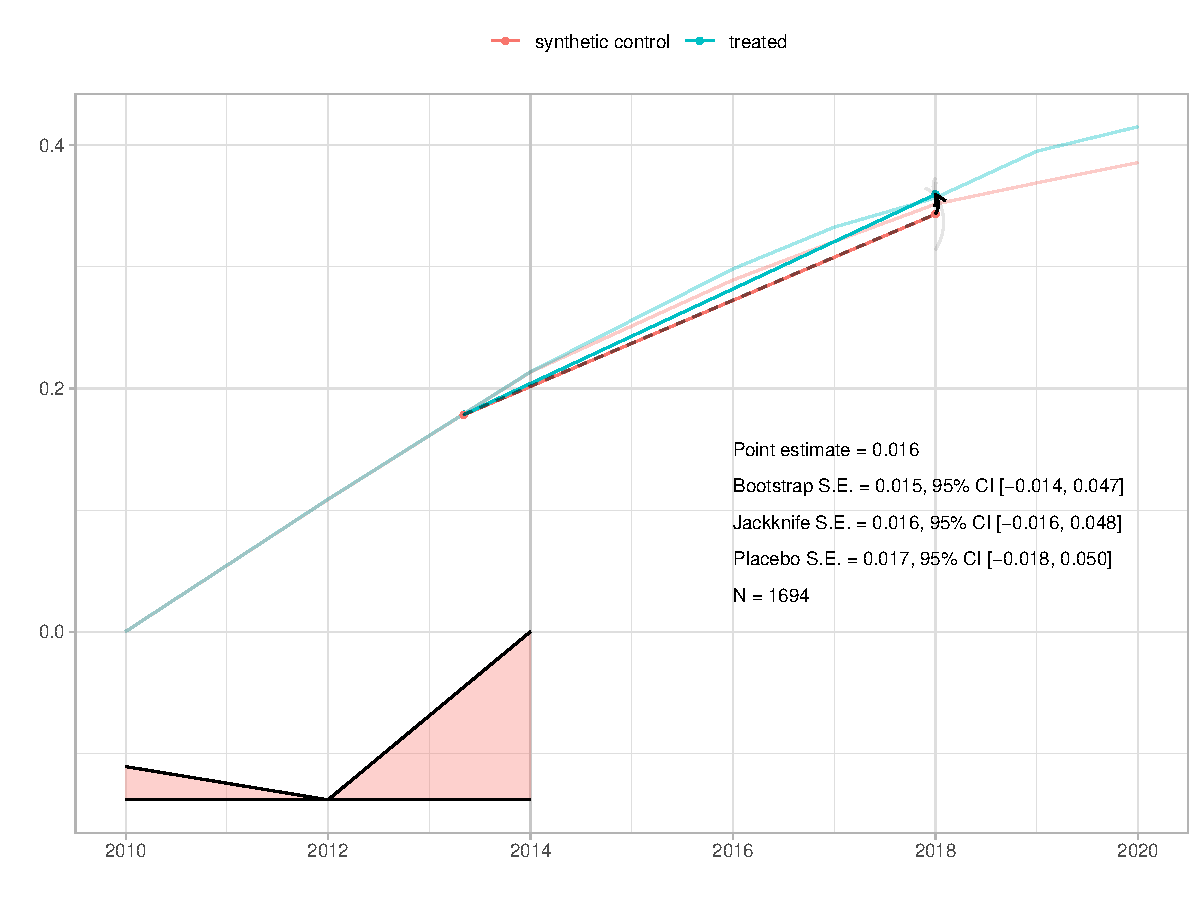
\includegraphics[width=0.7\linewidth]{Fig7.pdf}
    \caption{Brexit's Impact on Affiliate Exits (Synthetic DiD)}
    \label{fig:fig_SDiD-2}
    \end{center}

\footnotesize
\emph{Source:} Authors' compilation based on Toyo Keizai's OJC data.\\
\emph{Notes:} The figures show the results of synthetic DiD analysis based on the method of \cite{arkhangelsky2021synthetic}. 
The R \texttt{synthdid} package is used.  
We show trends in exit probability over time for Japanese affiliates in the UK and the relevant weighted average of control affiliates in other high-income EU countries, with the weights used to average pre-treatment periods shown as a shaded area at the bottom of the graphs. 
The blue lines indicate the treated group, while red line shows the control group.
The dashed line is the synthetic control.
The estimated effect is indicated by an arrow.
\end{minipage}

\end{figure}
% Fig7.Rmd
%%%%%%%%%%%%%%%%%%%%%%%%%%%%%%%%%%%%%%%%%%%%%%%%%%%%%%%%

Figure \ref{fig:fig_SDiD-2} shows the results of the SDiD analysis at the affiliate level.\footnote{We used \cite{synthdid}'s \texttt{synthdid} package.} 
The blue line presents the trends in exit probability over time for Japanese affiliates in the UK and the red line presents the relevant weighted average of control affiliates in other high-income EU countries.
The weights used to average pre-treatment periods are shown as the red-shaded areas at the bottom of the graph.\footnote{The control unit weights are aggregated at country-level and reported in \ref{sec:sdid_weights}.}
The estimated effect is indicated by an arrow.
The figure shows that the trends in exit probability for Japanese affiliates in the UK and the weighted average of control affiliates in other high-income EU countries are quite similar.
The point estimate of the effect of the Brexit referendum on the exit probability is 0.016, with a standard error of 0.017. Thus, the estimated effect of the referendum on the exit probability is negligible and insignificant, suggesting that the referendum period did not have a significant impact on the exit probability of Japanese affiliates in the UK. 

To ensure the robustness of our inference, we consider three standard error estimation methods for SDiD: Bootstrap, Jackknife, and Placebo. The Bootstrap method, which is the default for SDiD and is used to construct the confidence intervals in our plots, resamples all units (both treated and control) with replacement and re-estimates the entire SDiD algorithm. This approach captures both the uncertainty in weight estimation and the correlation structure within units, and it is recommended for its comprehensive coverage in finite samples \citep{arkhangelsky2021synthetic}. The Jackknife method, using a leave-one-out approach, provides a conservative coverage guarantee (Theorem 2 in \citealt{arkhangelsky2021synthetic}) even without homoskedasticity, provided the number of treated units is sufficiently large ($N_{tr} \gg 1$), as in our affiliate-level exit analysis. 

Finally, the Placebo method uses only the control group units to estimate the distribution of "fake" treatment effects under the assumption of homoskedasticity across units. However, in our setting, this assumption is likely violated. First, the outcome is binary ($exit_{it} \in \{0, 1\}$), where the variance $p(1-p)$ is a function of the mean; if exit rates differ between the UK and the rest of the EU, their variances will necessarily differ. Second, the common referendum shock creates cross-sectional correlation within the treatment group that the Placebo method fails to capture. In our estimation, while the Placebo SE is the smallest, the Bootstrap and Jackknife SEs also lead to the same conclusion: the effect of the Brexit referendum on exits is statistically indistinguishable from zero. This consistency reinforces the robustness of our finding that existing Japanese affiliates did not ``up sticks" following the referendum.


\subsection{Asset specificity}\label{sec:assetchannel}

Employing various empirical methods, we establish a robust finding: the Brexit referendum had negligible and statistically insignificant effects on Japanese FDI exits in the UK during the period we study. As outlined in our model in Section \ref{sec:Model}, the hysteresis effect of FDI significantly shapes firms' exit decisions. This effect implies that substantial sunk costs associated with FDI discourage firms from exiting, even when the host country becomes less attractive for investment. Consequently, affiliates in industries with higher asset specificity, which typically involve larger sunk costs, are expected to be less responsive to the referendum shock.

To elucidate the mechanism behind this hysteresis effect, we investigate the heterogeneous effects of the Brexit referendum on exit probability based on asset specificity. \cite{kermani2023asset} argue that high asset specificity is associated with less disinvestment and that the degree of asset specificity varies across industries. In our framework, we introduce asset specificity, denoted by $\rho_s \in (0, 1]$, where $\rho_s$ measures the degree to which investments in industry $s$ are sunk (i.e., non-recoverable). 

High $\rho_s$ (e.g., $\rho_s \to 1$) reflects industries with highly specific assets, such as specialized manufacturing plants, while low $\rho_s$ (e.g., $\rho_s \to 0$) characterizes industries with transferable assets, such as retail or generic office spaces. We incorporate $\rho_s$ into the incumbent's continuation condition. Following the logic of equation (\ref{eq:exit}), the condition for an incumbent firm ($FDI_{ih,t-1}=1$) to remain active in the host country is:
\begin{equation}
\pi_i(a_{ht}, \mathbf{z}_{it}) + \delta \left[ E_t \left( V_{ih,t+1} \mid FDI_{iht} = 1 \right) - E_t \left( V_{ih,t+1} \mid FDI_{iht} = 0 \right) \right] \geq -F_i^{Exit}(\rho_s),
\end{equation}
where $F_i^{Exit}(\rho_s)$ represents the effective exit cost, which increases with the degree of asset specificity $\rho_s$. 

As discussed in Section \ref{sec:Model}, Brexit reduces the current profitability $\pi_i$ and the expected future value $V_{ih,t+1}$ due to a decline in business conditions $a_{ht}$. However, for industries with high asset specificity ($\rho_s \approx 1$), the exit threshold $a_{ih}^{Exit}$ is significantly lowered (i.e., shifted to the left in Figure \ref{fig:band}). Furthermore, as shown in our uncertainty analysis, the increased probability of future deterioration ($\gamma > 0$) raises the option value of waiting, further insulating these firms from exit. In contrast, in industries with low asset specificity ($\rho_s \approx 0$), assets can be liquidated or repurposed more easily, resulting in a smaller $F_i^{Exit}$ and a higher exit threshold $a_{ih}^{Exit'}$. In these sectors, the same negative shock to $a_{ht}$ is more likely to trigger the exit condition.

This framework predicts that Brexit has minimal impact on FDI exits in high asset specificity industries due to the substantial hysteresis band, while it may significantly increase exits in low asset specificity industries where the band is narrower. To examine this, we utilize data from \cite{kermani2023asset} to categorize industries into those with low and high asset specificity. The classification procedure is detailed in \ref{sec:asset}.

We perform event study regressions for the subsamples of industries with low and high asset specificity. Figure \ref{fig:asset} presents the results of this analysis. As hypothesized, Figure \ref{fig:asset} shows that exit probabilities in low asset specificity industries (black line) rose significantly by the 2020 survey wave, while those in high asset specificity industries (red line) remained stable. Specifically, Brexit significantly increased the exit probability in low asset specificity industries by approximately 7\% in 2020 ($p < 0.05$), while it did not affect the exit probability in high asset specificity industries. These findings indicate that the hysteresis effect is stronger in industries with high asset specificity, aligning with prior studies by \cite{kermani2023asset} and \cite{kim2017asset}. Overall, our results substantiate the hypothesis that the interplay between sunk costs and policy uncertainty creates significant hysteresis, particularly when assets are highly industry-specific.


%%%%%%%%%%%%%%%%%%%%%%%%%%%%%%%%%%%%%%%%%%%%%%%%%%%%%%%%
\begin{figure}[ht]
\begin{center}

    \includegraphics[keepaspectratio, scale=0.6]{Fig8.eps}

 \caption{Asset specificity and Brexit's dynamic impact on exit probability}
    \label{fig:asset}
    
\end{center}

\footnotesize
\emph{Source:} Authors' compilation based on Toyo Keizai's OJC data.\\
\emph{Note:} The figures present the event study coefficients of the two-way fixed effects (TWFE) model with the 95\% confidence intervals. 
The figure draws the affiliate-level effects of the Brexit referendum on the exit probability.
The R \texttt{fixest} package is used.

\end{figure}
% Fig8.Rmd
%%%%%%%%%%%%%%%%%%%%%%%%%%%%%%%%%%%%%%%%%%%%%%%%%%%%%%%%



\section{The impacts on the new entry \label{sec:entry}}

So far, we have focused on the effect of the Brexit referendum on the exit behavior of incumbent Japanese affiliates in the UK. Across TWFE, ETWFE, pooled logit QMLE DiD, and SDiD specifications, the main result is that the referendum did not trigger a statistically meaningful increase in affiliate exits. This pattern is consistent with the hysteresis mechanism in our model: once sunk costs have been incurred, existing affiliates may remain in place even when expected profitability declines.

This makes the entry margin especially informative. Unlike incumbents, potential entrants can revise or postpone investment plans before committing sunk costs. In this section, we therefore examine whether the referendum and the uncertainty it generated discouraged new Japanese affiliate entry into the UK. The contrast between muted exit responses and weaker entry provides the clearest empirical test of the model's core prediction.

\subsection{Pooled Poisson QMLE DiD for Entry} \label{sec:PQMLE-entry}

To further validate the effect of the Brexit referendum on new affiliate entry while accounting for potential heterogeneous treatment effects across time and cohorts, we apply the pooled Poisson QMLE DiD specification proposed by \cite{wooldridge2023simple}. Given the count nature of our entry data, we estimate a pooled Poisson QMLE DiD model using the \texttt{jwdid} package in Stata. 

Table \ref{tab:entry2010combined} summarizes both the pooled Poisson event-study specification and the pooled Poisson QMLE DiD ATT estimates for the 2010--2020 sample. Columns (1) and (2) report the event-study coefficients from \texttt{ppmlhdfe}, while Columns (3) to (6) report the dynamic ATT estimates from \texttt{jwdid}. In the pooled Poisson QMLE DiD specifications, the coefficients directly represent log-scale Average Treatment Effects on the Treated (ATTs), that is, proportionate effects on new affiliate entry. Columns without covariates are paired with columns that add baseline controls fixed at their 2010 values, namely log GDP per capita, log distance from Japan, and median affiliate size in each host-country-industry cell in 2010. These controls allow us to adjust for cross-country differences in market size, geography, and pre-existing Japanese affiliate presence without introducing post-treatment controls \citep{wooldridge2023simple}.

To assess the validity of the conditional index parallel trends assumption, we also examine the pre-treatment leads in the pooled Poisson event-study specification. As shown by \citet{wooldridge2023simple}, under the canonical link for the linear exponential family, testing pre-trends in the pooled event-study model is algebraically equivalent to testing them using only untreated observations. We therefore use the pre-treatment coefficients in Columns (1) and (2) of Table \ref{tab:entry2010combined} as a diagnostic for the plausibility of the identifying assumption.

The estimates suggest that the Brexit referendum reduced new affiliate entry into the UK, especially in the post-referendum period. In the pooled Poisson event-study columns, the coefficients for 2016 and 2020 are negative, and the 2020 effect is large and precisely estimated. The pooled Poisson QMLE DiD ATT estimates from \texttt{jwdid} point in the same direction: the post-treatment ATTs are negative throughout, and the 2020 coefficient is again the largest in magnitude. Taken together, these results are consistent with the view that the referendum discouraged new entry by raising the expected cost of establishing new affiliates in the UK.

At the same time, Table \ref{tab:entry2010combined} also raises an identification concern. In the event-study specification, the coefficient on UK $\times$ Year 2010 is already negative and statistically significant, indicating that the UK and comparison countries were not evolving in parallel even before the referendum when the full 2010--2020 window is used. This casts doubt on the identifying assumptions underlying the pooled Poisson DiD interpretation. For this reason, we treat the pooled Poisson estimates as suggestive rather than definitive and turn next to the synthetic DiD approach, which is designed to reduce reliance on parallel trends by constructing a better pre-treatment comparison.


%%%%%%%%%%%%%%%%%%%%%%%%%%%%%%%%
{\renewcommand\normalsize{\scriptsize}%
\normalsize 
\begin{table}[!ht]\centering\caption{\label{tab:entry2010combined}The Brexit Referendum's Impact on New Affiliate Entry Count: PPML Event Study and Pooled Poisson QMLE (2010--2020)}\begin{threeparttable}\begin{tabular}{l*{6}{c}}\toprule
\multicolumn{1}{c}{} & \multicolumn{2}{c}{PPML Event Study} & \multicolumn{4}{c}{Pooled Poisson QMLE ATT} \\
\cmidrule(lr){2-3}\cmidrule(lr){4-7}
\multicolumn{1}{c}{} & \multicolumn{4}{c}{EU High-Income} & \multicolumn{2}{c}{All High-Income} \\
\cmidrule(lr){2-5}\cmidrule(lr){6-7}

                    &\multicolumn{1}{c}{(1)}&\multicolumn{1}{c}{(2)}&\multicolumn{1}{c}{(3)}&\multicolumn{1}{c}{(4)}&\multicolumn{1}{c}{(5)}&\multicolumn{1}{c}{(6)}\\
\midrule
~~UK $\times$ Year 2010 [ES]&      -0.381** &      -0.420** &               &               &               &               \\
                    &     (0.123)   &     (0.130)   &               &               &               &               \\
~~UK $\times$ Year 2012 [ES]&      -0.032   &      -0.019   &               &               &               &               \\
                    &     (0.160)   &     (0.199)   &               &               &               &               \\
~~UK $\times$ Year 2016 [ES]&      -0.368*  &      -0.378   &               &               &               &               \\
                    &     (0.181)   &     (0.198)   &               &               &               &               \\
~~UK $\times$ Year 2018 [ES]&      -0.116   &      -0.153   &               &               &               &               \\
                    &     (0.127)   &     (0.174)   &               &               &               &               \\
~~UK $\times$ Year 2020 [ES]&      -0.894***&      -0.837***&               &               &               &               \\
                    &     (0.189)   &     (0.192)   &               &               &               &               \\
~~UK $\times$ Year 2016 [ATT]&               &               &      -0.310   &      -0.513   &      -0.108   &      -0.338   \\
                    &               &               &     (0.175)   &     (0.386)   &     (0.173)   &     (0.281)   \\
~~UK $\times$ Year 2018 [ATT]&               &               &      -0.119   &      -0.014   &      -0.042   &      -0.218   \\
                    &               &               &     (0.135)   &     (0.346)   &     (0.093)   &     (0.181)   \\
~~UK $\times$ Year 2020 [ATT]&               &               &      -0.756***&      -0.800*  &      -0.375   &      -0.702** \\
                    &               &               &     (0.202)   &     (0.326)   &     (0.246)   &     (0.255)   \\
\midrule
Covariates          &          No   &         Yes   &          No   &         Yes   &          No   &         Yes   \\
Observations        &       2,868   &       1,290   &       1,319   &       1,277   &       2,347   &       2,290   \\
\bottomrule\end{tabular}\end{threeparttable}\par\medskip\parbox{\linewidth}{\footnotesize \textit{Notes:}  Columns (1)--(4) use EU high-income countries as the comparison group; Columns (5) and (6) include additional non-EU high-income countries (CAN, AUS, CHE, KOR, NZL). The outcome is the count of new Japanese affiliate entries into a host country by industry (biennial). Columns (1)--(2): PPML event study coefficients (\texttt{ppmlhdfe}) with year-sector fixed effects and a UK cohort dummy (GBR). Columns (3)--(6): dynamic ATT estimates from the pooled Poisson QMLE framework (\texttt{jwdid}; \citealt{wooldridge2023simple}). Reference year for PPML: 2014. Within each estimator, columns without and with covariates are estimated on the same sample retained by \texttt{ppmlhdfe}'s separation algorithm (no-covariate specification). Standard errors clustered at the country-by-industry level in parentheses. * $p<0.05$, ** $p<0.01$, *** $p<0.001$. }\end{table}

}
%%%%%%%%%%%%%%%%%%%%%%%%%%%%%%%%



\subsection{Synthetic DiD} \label{sec:SDiD-entry}

Figure~\ref{fig:fig_SDiD-entry} presents the results of the SDiD analysis at the industry level for new entry. It illustrates the trends in new entries of Japanese affiliates in the UK over time, compared to the weighted average of control affiliates in other high-income EU countries, also at the industry level. The weights used to compute the pre-treatment averages are shown by the shaded area at the bottom of the graph.\footnote{The control unit weights are aggregated at country-level and reported in \ref{sec:sdid_weights}.} The blue line represents the treated group, while the red line indicates the control group. The two lines closely track each other prior to the Brexit referendum, suggesting that the parallel trends assumption holds.
The dashed line depicts the synthetic control, and the estimated treatment effect is marked by an arrow in the figure. The results indicate that the Brexit referendum had a negative effect on new entry during the 2016--2020 uncertainty period, with a point estimate of $-0.145$ and a standard error of 0.052. This point estimate is economically meaningful, corresponding to approximately a 13.5\% reduction in new entries. However, the statistical significance of this result warrants careful interpretation. While the reported placebo-based standard error yields a significant result, this significance is sensitive to the estimation method. The placebo approach may underestimate uncertainty in this context, as the assumption of homoskedasticity is difficult to maintain for count variables like new entries, and cross-sectional correlations arising from the common referendum shock across industries may artificially inflate the statistical significance. Indeed, alternative standard error estimations using bootstrap or jackknife methods (not reported here) do not reach conventional significance levels. 

This sensitivity highlights the fragility of the statistical significance for the entry results. In synthetic DiD, there are three primary standard error estimation methods: Bootstrap, Jackknife, and Placebo. The Bootstrap method, which is the default for SDiD and is used for our plots, resamples across all units and captures both the systematic component of the referendum shock and the uncertainty in weight estimation. Similarly, the Jackknife method provides a conservative coverage guarantee even under heteroskedasticity. In our entry analysis, both of these more comprehensive methods yield lower statistical precision for the entry impact compared to the Placebo method. 

Finally, the Placebo method assumes that the distribution of "fake" treatment effects among control units accurately represents the uncertainty of the treatment effect. However, this method assumes homoskedasticity across units, which is difficult to maintain for count variables like new entries. Furthermore, it fails to account for the systematic referendum shock affecting all UK-based units simultaneously, which may artificially inflate the statistical significance. Thus, while our point estimate is substantial and consistent with the direction predicted by our model, the precision is limited, and the result should not be interpreted as definitive evidence of a statistically significant effect. 

Nevertheless, the overall pattern of results is highly informative. The clear asymmetry between the near-zero effect on exits (point estimate of 0.016, as shown in Figure~\ref{fig:fig_SDiD-2}) and the sizeable negative effect on entries aligns closely with our theoretical predictions. In our framework, sunk costs and policy uncertainty create a hysteresis band that makes existing affiliates more persistent than new entrants. The lower statistical precision for the entry results compared to the exit results is likely driven by the data structure: while the exit analysis utilizes affiliate-level data with a large number of observations, the entry analysis is conducted at the country-industry level, which significantly reduces the number of units and thus the statistical power. Despite these limitations, the overall pattern of results provides empirical support for the theoretical prediction that large policy shocks such as the Brexit referendum can asymmetrically affect the entry and exit margins of FDI. These results are also broadly consistent with the findings of \cite{breinlich2020} and \cite{cieslik2022brexit}.

%%%%%%%%%%%%%%%%%%%%%%%%%%%%%%%%%%%%%%%%%%%%%%%%%%%%%%%%
\begin{figure}[ht]
  \begin{minipage}{.95\linewidth}
  \begin{center}
  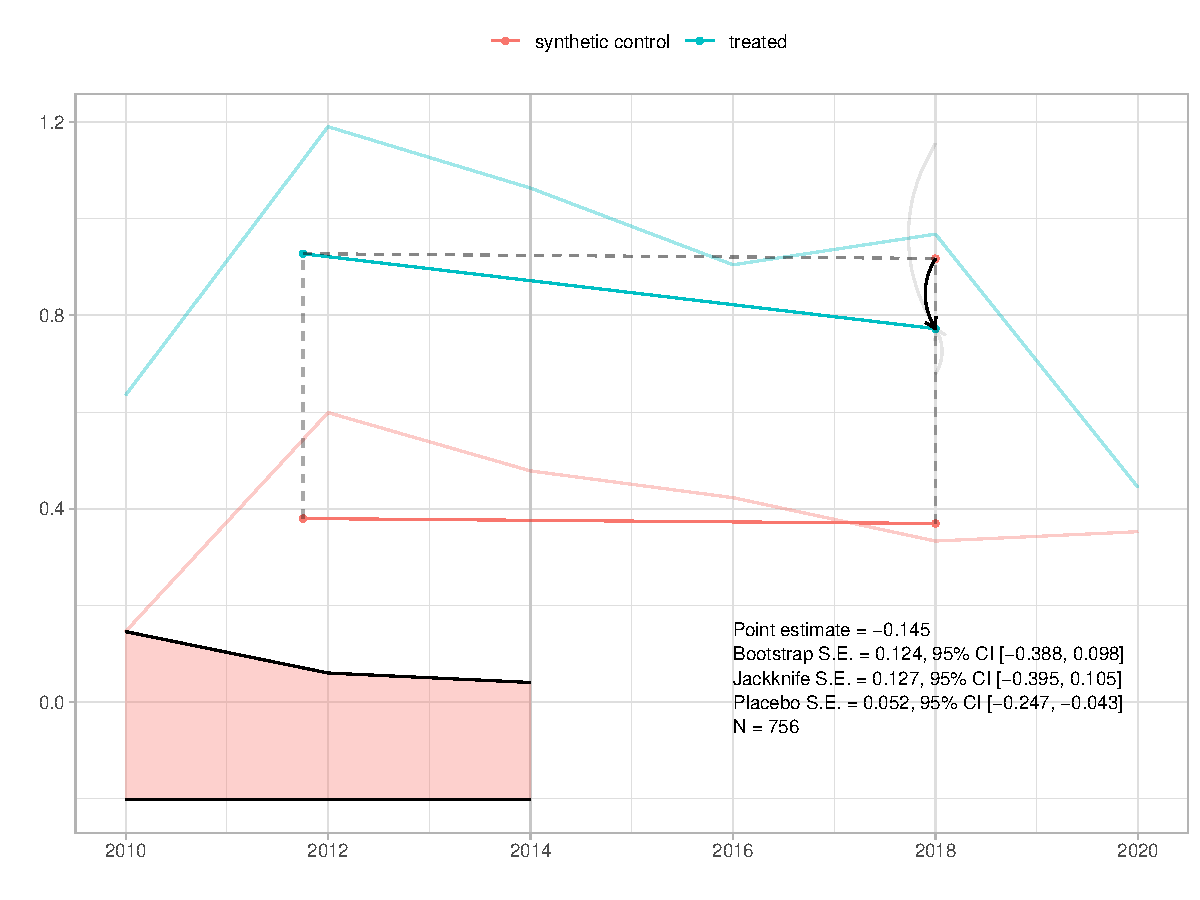
\includegraphics[width=0.7\linewidth]{Fig9.pdf}
  \caption{Brexit's Impact on New Affiliate Entries (Synthetic DiD)}
  \label{fig:fig_SDiD-entry}
  \end{center}

\footnotesize
\emph{Source:} Authors' compilation based on Toyo Keizai's OJC data.\\
\emph{Notes:} The figures show the results of synthetic DiD analysis based on the method of \cite{arkhangelsky2021synthetic}. 
The R \texttt{synthdid} package is used.  
We show trends in new entry over time for Japanese affiliates in the UK and the relevant weighted average of control affiliates in other high-income EU countries at the industry level, with the weights used to average pre-treatment periods shown as a shaded area at the bottom of the graphs. 
The blue lines indicate the treated group, while red line shows the control group.
The dashed line is the synthetic control.
The estimated effect is indicated by an arrow.
\end{minipage}

\end{figure}
%%%%%%%%%%%%%%%%%%%%%%%%%%%%%%%%%%%%%%%%%%%%%%%%%%%%%%%%
\section{Conclusion\label{sec:conclusion}}

This paper presents a theoretical model incorporating sunk costs and policy uncertainty to understand affiliate exit and entry, and empirically examines how the Brexit referendum and the subsequent uncertainty period affected Japanese affiliates in the UK. Utilizing Toyo Keizai Inc.’s Overseas Japanese Companies Data from two-year survey waves between 2010 and 2020, we employ various difference-in-differences and synthetic difference-in-differences methods to assess both the exit probability of existing affiliates and the entry margin for new affiliates relative to other European host countries. The central empirical result is an asymmetry between these two margins. Existing affiliates do not exit the UK at a statistically meaningful higher rate after the referendum, whereas new affiliate entry appears to decline. This pattern aligns with our model’s prediction that hysteresis in foreign direct investment---driven jointly by sunk costs and the option value of waiting under policy uncertainty---primarily stabilizes incumbent affiliates while discouraging new commitments.

Policymakers can capitalize on hysteresis by offering targeted incentives to existing affiliates, such as tax breaks or regulatory stability, to maintain FDI stocks during policy shocks. These findings also inform future customs union exits, highlighting the need to address sunk cost barriers and manage policy uncertainty to mitigate FDI declines.

It is crucial to consider the broader context of Japanese FDI in the UK. Notably, our data show that the number of Japanese affiliates in the UK began to level off well before the Brexit referendum, accompanied by increased investment in the rest of the EU. On the one hand, the findings of this paper indicate that the ``upping sticks" phenomenon feared by the Japanese government in 2016 did not materialize among existing affiliates during the referendum-to-exit period. On the other hand, our entry analysis indicates that the referendum likely reduced new Japanese FDI entries into the UK, with the SDiD point estimate implying approximately a 13.5\% decline. While the statistical significance of this entry effect is sensitive to the estimation method for standard errors, its magnitude is economically meaningful. Taken together, these results suggest that the decline in Japanese investment in the UK during the referendum period was driven more by weaker entry than by stronger exit.


Future research could extend the FDI model presented in this paper by incorporating firm heterogeneity, as in \citet{graziano2021brexit} for exporting. Investigating how firm heterogeneity interacts with the sunk cost hysteresis and option value mechanisms identified here would be a promising avenue for further study.
Another natural extension would be to allow for intermediate adjustment margins, such as partial divestiture or ownership restructuring, rather than restricting firms to the extensive-margin choices of staying, exiting, or entering. Such an extension could help connect the sunk-cost mechanism developed here to more gradual forms of affiliate adjustment during periods of policy uncertainty.

Research could also extend the analysis to other foreign investors in the UK to assess whether the observed hysteresis effects apply to firms from different countries. Additionally, future work might examine referendum-related exits beyond 2020. While incorporating data from the COVID-affected years (2021, 2022, and beyond) may seem valuable, doing so would likely introduce confounding factors that obscure the specific effects of the referendum-induced uncertainty on Japanese FDI. Disentangling the impact of the pandemic would require a separate analytical approach and lies beyond the scope of the present study. Nevertheless, future work could explore the interaction between Brexit and the pandemic to better understand their combined effects on investment behavior.
Finally, the UK–Japan Comprehensive Economic Partnership Agreement, as well as trade and investment arrangements between the UK and the EU, remained uncertain during the period under study. The extent to which these agreements have helped retain Japanese affiliates in the UK remains an open question for future research.

\section*{Acknowledgments}
\noindent We are grateful to Stefania Garetto and anonymous referees for their constructive comments and suggestions, which greatly improved the paper.
We also thank Tamae Kawasaki for her invaluable guidance on the imputation methods.
Tanaka acknowledges financial support from the Japan Society for the Promotion of Science (JSPS): KAKENHI Grant Number JP19K01612 and JP23K01356. The usual disclaimer applies.

\vspace{0.5cm}
\noindent
\textbf{Data availability statement}
The Overseas Japanese Companies (OJC) data used in this study were purchased from Toyo Keizai Inc. and are subject to license restrictions. Therefore, the data cannot be made publicly available by the authors. The code used to reproduce the tables and figures in this paper will be made publicly available.
\newline
\textbf{Funding statement}
Tanaka acknowledges financial support from JSPS's Grants-in-Aid for Scientific Research (No. 19K01612 and 23K01356).
\newline
\textbf{Conflict of interest disclosure}
The authors declare no conflicts of interest.

%%%%%%%%%%%%%%%%%%%%%%%%%%%%%%%%%%%%%%%%%%%%%%%%%
%\clearpage
%\begin{singlespace}
%\bibliographystyle{plainnat}
%\bibliographystyle
%\bibliographystyle{apalike}
%\bibliographystyle{aer}
%\bibliographystyle{jpe}
%\bibliographystyle{econ-econometrica}
\bibliographystyle{econ-aea}
\bibliography{brexit_ref}
%\end{singlespace}
%%%%%%%%%%%%%%%%%%%%%%%%%%%%%%%%%%%%%%%%%%%%%%%%%



%%%%%%%%%%%%%%%%%%%%%%%%%%%%%%%%%%%%%%%%%%%%%%%%%
%%%%% These commands start the appendix and change the Table & Figure numbering
\newpage
\appendix
\setcounter{table}{0}
\renewcommand{\tablename}{Appendix Table}
\renewcommand{\figurename}{Figure}
\renewcommand{\thetable}{A\arabic{table}}
\setcounter{figure}{0}
\renewcommand{\thefigure}{A\arabic{figure}}
%%%%%%%%%%%%%%%%%%%%%%%%%%%%%%%%%%%%%%%%%%%%%%%%%


%\begin{appendices}

\appendix
\newpage 
\section*{Appendices}


\section{Country list}\label{country}

Table \ref{tab:country-list} reports the number of observations by host country.
We only use foreign affiliates in which Japanese parent firms own more than 10\% of the equity.
For the empirical analysis, we restrict the sample to affiliates that existed in 2010, constructing a balanced panel spanning the two-year survey waves from 2010 to 2020.
Accordingly, the number of observations for each host country in Table \ref{tab:country-list} equals the number of affiliates in 2010 multiplied by six survey years of data (2010, 2012, 2014, 2016, 2018, and 2020).

%%%%%%%%%%%%%%%%%%%%%%%%%%%%%%%%
{\renewcommand\normalsize{\scriptsize}%
\normalsize 
\begin{table}[!ht]
\centering
\caption{\label{tab:country-list}Country list.}
\centering
\begin{threeparttable}
\begin{tabular}[t]{llllll}
\hline
\multicolumn{3}{c}{High-income EU} & \multicolumn{3}{c}{Middle-income EU} \\
\cline{1-3} \cline{4-6}
Country & N of observations & N of affiliates & Country & N of observations & N of affiliates\\
\hline
Austria & 144 & 18 & Bulgaria & 24 & 3\\
Belgium & 760 & 95 & Czechia & 400 & 50\\
Denmark & 128 & 16 & Greece & 48 & 6\\
Finland & 88 & 11 & Hungary & 256 & 32\\
France & 1584 & 198 & Poland & 280 & 35\\
Germany & 3520 & 440 & Portugal & 112 & 14\\
Ireland & 168 & 21 & Romania & 72 & 9\\
Italy & 752 & 94 & Slovakia & 80 & 10\\
Luxembourg & 80 & 10 & Slovenia & 24 & 3\\
Netherlands & 2128 & 266 & Spain & 576 & 72\\
Sweden & 232 & 29 &  &  & \\
United Kingdom & 3968 & 496 &  &  & \\
\hline
\end{tabular}
\begin{tablenotes}
\item \textit{Note: } 
\item This table shows the number of observations ($=$ the number of affiliates in 2010 $\times$ eight years) by the host country. The sample includes the Japanese affiliates in the EU. Sample restricted to affiliates with $>10$\% Japanese ownership.
\end{tablenotes}
\end{threeparttable}
\end{table}

}
% TabA1_B2.Rmd
% Currently aligned to the hand-tuned layout while TabA1_B2.Rmd is being updated.
% tab:country-list
%%%%%%%%%%%%%%%%%%%%%%%%%%%%%%%%



\clearpage
\section{Descriptive statistics}\label{descriptive}

Table \ref{tab:desc} presents the descriptive statistics of variables used in the main analysis.



%%%%%%%%%%%%%%%%%%%%%%%%%%%%%%%%
{\renewcommand\normalsize{\scriptsize}%
\normalsize 
\begin{table}[!ht]
\centering
\begin{talltblr}[         %% tabularray outer open
caption={Descriptive statistics. \label{tab:desc}},
note{}={This table shows the descriptive statistics of the estimation sample. The sample includes the Japanese affiliates in the EU. The variable ``Number of affiliates in EU'' is the number of affiliates in the EU. The variable ``Affiliate size'' is the size of the affiliate. The variable ``High-income EU'' is a dummy variable that takes 1 if the affiliate is located in the high-income EU countries. The variable ``Exit'' is a dummy variable that takes 1 if the affiliate exits the host country. The variable ``Sector'' is the sector of the affiliate.},
]                     %% tabularray outer close
{                     %% tabularray inner open
colspec={Q[]Q[]Q[]Q[]Q[]Q[]Q[]Q[]},
hline{3}={1-8}{solid, black, 0.05em},
hline{7}={1-8}{solid, black, 0.05em},
hline{2}={3,5}{solid, black, 0.05em, l=-0.5},
hline{2}={4,6}{solid, black, 0.05em, r=-0.5},
hline{1}={1-8}{solid, black, 0.1em},
hline{15}={1-8}{solid, black, 0.1em},
cell{1}{1}={}{halign=c},
cell{1}{2}={}{halign=c},
cell{1}{3}={c=2}{halign=c},
cell{1}{4}={}{halign=c},
cell{1}{5}={c=2}{halign=c},
cell{1}{6}={}{halign=c},
cell{1}{7}={}{halign=c},
cell{1}{8}={}{halign=c},
cell{2-14}{1}={}{halign=l},
cell{2-14}{2}={}{halign=l},
cell{2-14}{3}={}{halign=r},
cell{2-14}{4}={}{halign=r},
cell{2-14}{5}={}{halign=r},
cell{2-14}{6}={}{halign=r},
cell{2-14}{7}={}{halign=r},
cell{2-14}{8}={}{halign=r},
}                     %% tabularray inner close
&  & a. UK (N=3968) &  & b. Other EU (N=11456) &  &  &  \\
&    & Mean & Std. Dev. & Mean & Std. Dev. & Diff. in Means & Std. Error \\
Number of affiliates in EU &  & \num{5.1} & \num{6.6} & \num{5.2} & \num{6.2} & \num{0.1} & \num{0.1} \\
Affiliate size &  & \num{164.0} & \num{695.5} & \num{163.8} & \num{625.6} & \num{-0.2} & \num{12.5} \\
Japanese ownership ratio &  & \num{0.7} & \num{0.4} & \num{0.7} & \num{0.4} & \num{-0.0} & \num{0.0} \\
Year &  & \num{2015.8} & \num{3.3} & \num{2015.8} & \num{3.3} & \num{0.0} & \num{0.1} \\
&  & N & Pct. & N & Pct. &  &  \\
High-income EU & High-income EU & \num{3968} & \num{100.0} & \num{9584} & \num{83.7} &  &  \\
& Other EU & \num{0} & \num{0.0} & \num{1872} & \num{16.3} &  &  \\
Exit dummy & Exit & \num{1052} & \num{26.5} & \num{3001} & \num{26.2} &  &  \\
& Survive & \num{2916} & \num{73.5} & \num{8455} & \num{73.8} &  &  \\
Sector & Agriculture \& Mining & \num{88} & \num{2.2} & \num{96} & \num{0.8} &  &  \\
& Manufacturing & \num{872} & \num{22.0} & \num{3080} & \num{26.9} &  &  \\
& Services & \num{3008} & \num{75.8} & \num{8280} & \num{72.3} &  &  \\
\end{talltblr}
\end{table}

}
% TabA1_B2.Rmd
% \caption{Descriptive statistics}\label{tab:Des}
%%%%%%%%%%%%%%%%%%%%%%%%%%%%%%%%


\clearpage
\section{Location of Japanese affiliates in Europe before and after the Brexit referendum}\label{map}


Figure \ref{fig:map} illustrates the distribution of Japanese multinational firms across Europe in 2010 and 2020, highlighting the number of Japanese affiliates in each country.
In 2010, the leading destinations for Japanese firms in Europe were the UK (496 affiliates), followed by Germany (440), the Netherlands (266), and France (198).
By 2020, the number of affiliates in the UK had slightly increased to 503, while Germany experienced a significant rise to 534.
The Netherlands and Italy also saw moderate increases—from 266 to 290 and from 94 to 103 affiliates, respectively—whereas France experienced a slight decline, from 198 to 186.
Overall, the figure shows that while the UK remained the second most popular destination for Japanese firms in Europe, the growth in the number of affiliates there was modest compared to the substantial increase observed in Germany.


%%%%%%%%%%%%%%%%%%%%%%%%%%%%%%%%%%%%%%%%%%%%%%%%%%%%%%%%
\begin{figure}[ht]
\begin{center}

    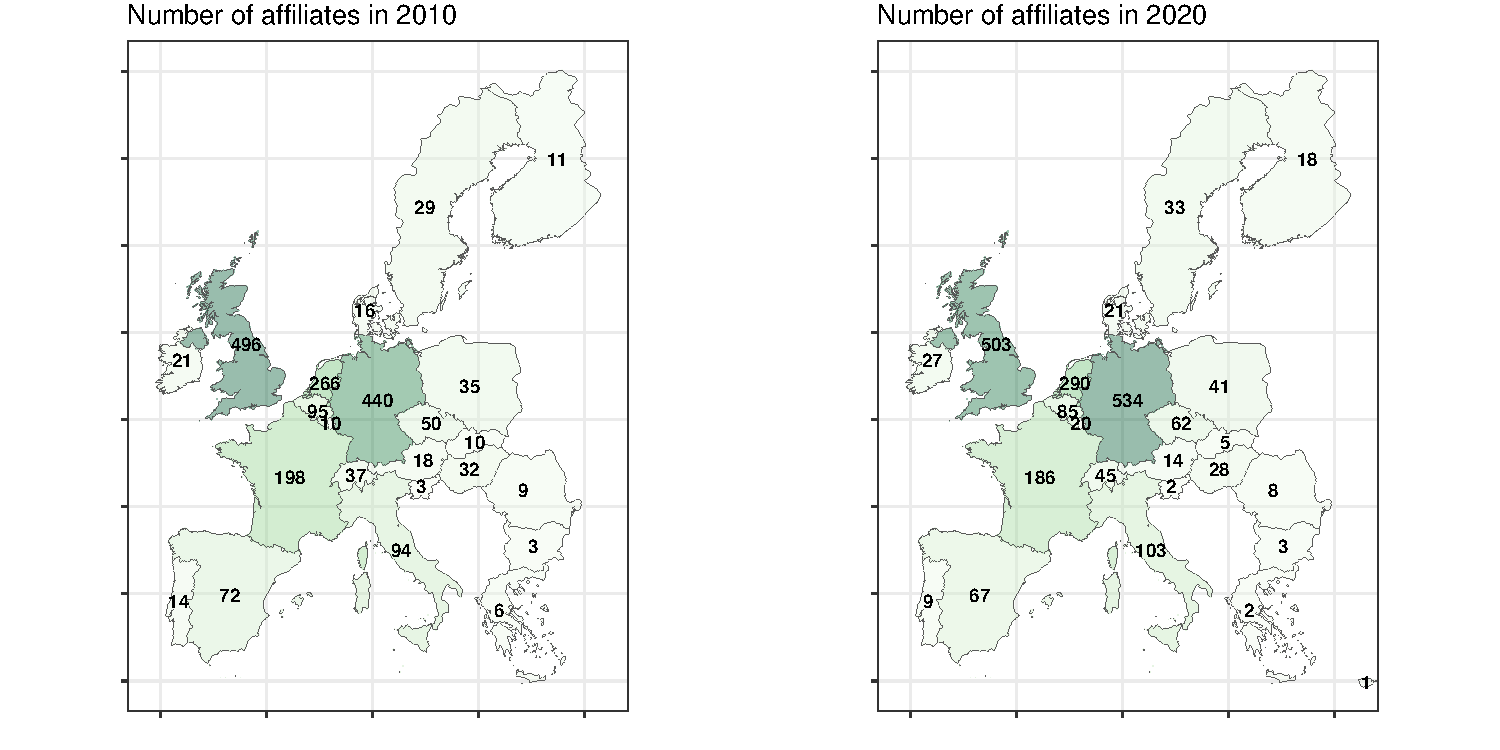
\includegraphics[keepaspectratio, width=\textwidth]{FigC1.pdf}

  \caption{Location of Japanese affiliates in Europe}
    \label{fig:map}

\end{center}

\footnotesize
\emph{Source:} Authors' compilation based on Toyo Keizai's OJC data.\\
\emph{Note:}
The figure shows the number of Japanese affiliates in European countries.

\end{figure}
% FigC1.Rmd
%%%%%%%%%%%%%%%%%%%%%%%%%%%%%%%%%%%%%%%%%%%%%%%%%%%%%%%%



\clearpage
\section{Synthetic DiD Control Unit Weights}\label{sec:sdid_weights}

Table \ref{tab:sdid_weights} reports the synthetic DiD control unit weights aggregated by country, corresponding to the SDiD estimates shown in Figure \ref{fig:fig_SDiD-2} (affiliate exits) and Figure \ref{fig:fig_SDiD-entry} (new affiliate entries).


%%%%%%%%%%%%%%%%%%%%%%%%%%%%%%%%
{\renewcommand\normalsize{\scriptsize}%
\normalsize 
\begin{table}[!h]
\centering
\caption{\label{tab:sdid_weights}Synthetic DiD Control Unit Weights by Country}
\centering
\begin{tabular}[t]{lrr}
\toprule
Country & Exit & Entry\\
\midrule
Austria & 0.0150 & 0.0751\\
Belgium & 0.0792 & 0.0814\\
Denmark & 0.0135 & 0.0735\\
Finland & 0.0092 & 0.0796\\
France & 0.1652 & 0.1200\\
\addlinespace
Germany & 0.3669 & 0.1284\\
Ireland & 0.0177 & 0.0800\\
Italy & 0.0785 & 0.1001\\
Luxembourg & 0.0083 & 0.0799\\
Netherlands & 0.2220 & 0.1094\\
\addlinespace
Sweden & 0.0245 & 0.0727\\
\bottomrule
\end{tabular}
\end{table}

}
% TabD3.Rmd
%%%%%%%%%%%%%%%%%%%%%%%%%%%%%%%%




\clearpage
\section{Asset Specificity}\label{sec:asset}

\cite{kermani2023asset} construct a novel dataset to measure asset specificity among nonfinancial firms, focusing on liquidation recovery rates (liquidation value relative to book value) across major industries. Using U.S. Chapter 11 bankruptcy filings from 2000 to 2018, they estimate that the average liquidation recovery rate for property, plant, and equipment (PPE) is 35\% (standard deviation 13\%).
They find that asset specificity, driven by physical attributes like mobility, customization, and durability, varies significantly across industries and impacts investment irreversibility, uncertainty effects.

\cite{kermani2023asset} provide a comprehensive dataset on liquidation recovery rates across industries. 
We assign the liquidation recovery rates from their Table II to the industries in the OJC dataset based on corresponding SIC codes. For OJC industries associated with multiple SIC codes, we calculate the average of the liquidation recovery rates of the relevant SIC codes. Following \cite{kermani2023asset}, who report an average PPE liquidation recovery rate of 0.35, we define industries with liquidation recovery rates above 0.35 as having low asset specificity, and those below 0.35 as having high asset specificity. This classification allows us to analyze the role of asset specificity within the OJC dataset.
Tables \ref{tab:SpecificityHigh} and \ref{tab:SpecificityLow} present the list of industries with high and low asset specificity, respectively.




%%%%%%%%%%%%%%%%%%%%%%%%%%%%%%%%
{\renewcommand\normalsize{\scriptsize}%
\normalsize 
\begin{table}[ht]
\centering
\caption{Industry Liquidation Recovery Rates with High Asset Specificity}
\label{tab:SpecificityHigh}
\centering
\begin{threeparttable}
\begin{tabular}{llccc}
\toprule
\textbf{Code} & \textbf{Industry} & \textbf{Liquidation Recovery Rate} & \textbf{Asset Specificity} & \textbf{SIC} \\
\midrule
1210 & Construction & 0.325 & High & 15, 17 \\
1410 & Textiles, Apparel & 0.340 & High & 22, 23 \\
1510 & Pulp, Paper & 0.310 & High & 26 \\
1610 & Chemicals & 0.240 & High & 28 \\
1710 & Pharmaceuticals & 0.240 & High & 28 \\
2510 & Electrical Machinery & 0.350 & High & 36 \\
2810 & Other Manufacturing & 0.270 & High & 39 \\
3510 & Communications, Broadcasting & 0.240 & High & 48 \\
3610 & Newspapers, Publishing & 0.310 & High & 27 \\
3710 & Video, Music & 0.310 & High & 78 \\
3810 & Advertising & 0.310 & High & 73 \\
3910 & Information, Systems, Software & 0.310 & High & 73 \\
4610 & Glass, Stone \& Clay Products Wholesale & 0.330 & High & 50 \\
4710 & Iron \& Steel, Metals Wholesale & 0.330 & High & 50 \\
4810 & Machinery Wholesale & 0.330 & High & 50 \\
4910 & Electrical Machinery Wholesale & 0.330 & High & 50 \\
5010 & Transportation Equipment Wholesale & 0.330 & High & 50 \\
5110 & Precision Instruments Wholesale & 0.330 & High & 50 \\
5310 & Department Stores & 0.310 & High & 53 \\
5510 & Specialty Stores & 0.173 & High & 56, 57, 59 \\
5610 & Automobile Sales & 0.040 & High & 55 \\
5710 & Other Retail & 0.280 & High & 59 \\
5810 & Eating \& Drinking Places, Food Service & 0.190 & High & 58 \\
7210 & Travel & 0.230 & High & 72 \\
7310 & Leisure, Entertainment & 0.210 & High & 79 \\
7410 & Consulting & 0.310 & High & 73, 87 \\
7510 & Architectural Design & 0.310 & High & 87 \\
7610 & Human Resources, Contract Services & 0.310 & High & 73 \\
7710 & Building Management, Security Services & 0.270 & High & 73, 72 \\
7810 & Machinery Repair, etc. & 0.310 & High & 73 \\
7910 & Other Services & 0.283 & High & 72, 73, 87 \\
8010 & Holding Companies & 0.310 & High & 73 \\
\bottomrule
\end{tabular}


\begin{tablenotes}
\item \textit{Notes: } 
 The liquidation recovery rates from Table II of \cite{kermani2023asset} were assigned to the industries in the OJC data corresponding to their SIC codes. For industries in the OJC data that correspond to multiple SIC codes, the average value of the liquidation recovery rates of the relevant SIC codes was used. Industries with liquidation recovery rates exceeding the average value of 0.35 are defined as having low asset specificity, while those below this threshold are defined as having high asset specificity.
 \end{tablenotes}
\end{threeparttable}

\end{table}
}
% TabE4_E5.do
% /Users/ayumu/Documents/GitHub/2024Brexit/01_code/04_stata/
%%%%%%%%%%%%%%%%%%%%%%%%%%%%%%%%


%%%%%%%%%%%%%%%%%%%%%%%%%%%%%%%%
{\renewcommand\normalsize{\scriptsize}%
\normalsize 
\begin{table}[ht]
\centering
\caption{Industry Liquidation Recovery Rates with Low Asset Specificity}
\label{tab:SpecificityLow}
\centering
\begin{threeparttable}
\begin{tabular}{llccc}
\toprule
\textbf{Code} & \textbf{Industry} & \textbf{Liquidation Recovery Rate} & \textbf{Asset Specificity} & \textbf{SIC} \\
\midrule
1110 & Mining & 0.390 & Low & 10, 12, 13, 14 \\
1310 & Food Products & 0.370 & Low & 20 \\
1810 & Petroleum, Coal & 0.360 & Low & 13, 12 \\
1910 & Rubber Products & 0.430 & Low & 30 \\
2010 & Glass, Stone \& Clay Products & 0.440 & Low & 32 \\
2110 & Iron \& Steel & 0.430 & Low & 33 \\
2210 & Non-ferrous Metals & 0.430 & Low & 33 \\
2310 & Metal Products & 0.390 & Low & 34 \\
2410 & Machinery & 0.360 & Low & 35 \\
2610 & Transportation Equipment & 0.380 & Low & 37 \\
2710 & Precision Instruments & 0.380 & Low & 38 \\
2910 & Electric Power, Gas & 0.500 & Low & 49 \\
3010 & Railway, Bus & 0.540 & Low & 41 \\
3110 & Freight Transport & 0.540 & Low & 42 \\
3210 & Shipping & 0.490 & Low & 44 \\
3310 & Air Transport & 0.510 & Low & 45 \\
3410 & Warehousing, Logistics-related & 0.580 & Low & 47, 42 \\
4010 & General Wholesale & 0.435 & Low & 50, 51 \\
4110 & Textiles, Apparel Wholesale & 0.540 & Low & 51 \\
4210 & Food Products Wholesale & 0.540 & Low & 51 \\
4310 & Chemicals Wholesale & 0.540 & Low & 51 \\
4410 & Pharmaceuticals Wholesale & 0.540 & Low & 51 \\
4510 & Petroleum, Fuel Wholesale & 0.540 & Low & 51 \\
5210 & Other Wholesale & 0.435 & Low & 50, 51 \\
5410 & Supermarkets & 0.360 & Low & 54 \\
7110 & Hotels & 0.500 & Low & 70 \\
\bottomrule
\end{tabular}

\begin{tablenotes}
\item \textit{Notes: } 
 The liquidation recovery rates from Table II of \cite{kermani2023asset} were assigned to the industries in the OJC data corresponding to their SIC codes. For industries in the OJC data that correspond to multiple SIC codes, the average value of the liquidation recovery rates of the relevant SIC codes was used. Industries with liquidation recovery rates exceeding the average value of 0.35 are defined as having low asset specificity, while those below this threshold are defined as having high asset specificity.
 \end{tablenotes}
\end{threeparttable}
\end{table}

}
% TabE4_E5.do
% /Users/ayumu/Documents/GitHub/2024Brexit/01_code/04_stata/
%%%%%%%%%%%%%%%%%%%%%%%%%%%%%%%%



\clearpage
\section{Affiliate-level exit responses by parent-level UK exposure}\label{sec:parent_uk_exposure}

This appendix reports an additional heterogeneity exercise based on parent-level UK exposure. The main text shows that the average effect of the Brexit referendum on affiliate exit is close to zero, consistent with the hysteresis mechanism in our model. At the same time, the model also implies that affiliates facing a larger decline in expected profitability should exhibit a stronger exit response, even when sunk costs dampen adjustment on average. To examine this margin, we ask whether affiliate-level exit responses were larger for affiliates whose parent firms were more exposed to the UK before the referendum.

For this heterogeneity exercise, we construct parent-level UK exposure using the share of each parent firm’s affiliates located in the UK in 2010. Among parent firms with any UK presence, the median UK affiliate share is 0.125. We classify affiliates as belonging to the high-exposure group if their parent firm’s 2010 UK affiliate share is weakly above this threshold, and to the low-exposure group otherwise. In the baseline exit sample, the high-exposure group contains 199 parent firms and 313 affiliates, while the low-exposure group contains 182 parent firms and 720 affiliates. For comparison, the group of parents with no UK exposure contains 519 parent firms and 661 affiliates.

Within each group, we estimate the same affiliate-level TWFE event-study specification used in the baseline analysis, with year and affiliate fixed effects, and cluster standard errors at the country level. Figure \ref{fig:parent_uk_exposure} plots the resulting event-study coefficients for exit probability.
The results show that the estimated Brexit effect on affiliate exit is larger for affiliates whose parent firms had higher pre-referendum UK exposure. This pattern is consistent with the model once we allow the referendum shock to vary in intensity across firms: parents with greater UK exposure likely experienced a larger decline in expected profitability, so affiliates belonging to those parents display a stronger exit response, even though the average exit effect in the full sample remains small. 


%%%%%%%%%%%%%%%%%%%%%%%%%%%%%%%%%%%%%%%%%%%%%%%%%%%%%%%%
\begin{figure}[ht]
\begin{center}

    \includegraphics[keepaspectratio, scale=0.6]{FigF2.eps}

  \caption{Affiliate-level exit responses by parent-level UK exposure}
    \label{fig:parent_uk_exposure}

\end{center}

\footnotesize
\emph{Source:} Authors' compilation based on Toyo Keizai's OJC data.\\
\emph{Note:}
Low UK exposure: N = 5760, Parent firms = 182, Affiliates = 720, Observations = 5760.\\
High UK exposure: N = 2504, Parent firms = 199, Affiliates = 313, Observations = 2504.

\end{figure}
% FigF2.Rmd
%%%%%%%%%%%%%%%%%%%%%%%%%%%%%%%%%%%%%%%%%%%%%%%%%%%%%%%%


\clearpage
\section{Affiliate-level exit responses by the number of UK affiliates within parent firms}\label{sec:multi_uk_affiliates}

This appendix also reports a heterogeneity exercise based on whether a parent firm had only one UK affiliate or two or more UK affiliates in 2010. This split is motivated by the possibility that parent firms with multiple UK affiliates may have greater scope to reorganize within the UK after the referendum, for example by closing one affiliate while retaining other UK operations. To examine this possibility, we divide affiliates according to the number of UK affiliates held by their parent firm in 2010 and estimate the same affiliate-level TWFE event-study specification as in the baseline analysis, with year and affiliate fixed effects and standard errors clustered at the country level.

In the sample, 381 parent firms have at least one UK affiliate in 2010. Among them, 55 parent firms have two or more UK affiliates. The group of parents with one UK affiliate contains 326 parent firms, 689 affiliates, and 4,134 affiliate-period observations. The group of parents with two or more UK affiliates contains 55 parent firms, 344 affiliates, and 2,064 affiliate-period observations. For comparison, the group of parents with no UK affiliates contains 519 parent firms, 661 affiliates, and 3,966 affiliate-period observations.

Figure \ref{fig:multi_uk_affiliates} reports the resulting event-study coefficients. The estimates do not indicate that affiliates belonging to parents with multiple UK affiliates were more likely to exit after the referendum. If anything, the post-referendum coefficients are negative for the group whose parents had two or more UK affiliates in the UK. At the same time, the pre-treatment coefficients for that group are also statistically different from zero, so the pattern should be interpreted cautiously rather than as strong causal evidence. A plausible interpretation is that parent firms with multiple UK affiliates may have had more flexibility to reorganize internally while preserving some UK presence, which could reduce the need for full affiliate exit.


%%%%%%%%%%%%%%%%%%%%%%%%%%%%%%%%%%%%%%%%%%%%%%%%%%%%%%%%
\begin{figure}[ht]
\begin{center}

    \includegraphics[keepaspectratio, scale=0.6]{FigG3.eps}

  \caption{Affiliate-level exit responses by the number of UK affiliates within parent firms}
    \label{fig:multi_uk_affiliates}

\end{center}

\footnotesize
\emph{Source:} Authors' compilation based on Toyo Keizai's OJC data.\\
\emph{Notes:} One UK affiliate: N = 5512, Parent firms = 326, Affiliates = 689, Observations = 5512.\\
Two or more UK affiliates: N = 2752, Parent firms = 55, Affiliates = 344, Observations = 2752.

\end{figure}
% FigG3.Rmd
%%%%%%%%%%%%%%%%%%%%%%%%%%%%%%%%%%%%%%%%%%%%%%%%%%%%%%%%

\clearpage
\section{Exit and entry responses by Brexit MFN risk exposure}\label{sec:mfn_risk}

This appendix examines whether the effects of the Brexit referendum on affiliate exit probability and new affiliate entry differ across industries classified by their exposure to potential MFN tariff risk. The classification follows \citet{graziano2021brexit}, who show that Brexit uncertainty had stronger effects in sectors facing higher potential MFN tariffs in the event of a hard Brexit.

We classify each affiliate into one of three groups using the affiliate sector code recorded in the Toyo Keizai OJC data, matched to the sector-level MFN risk estimates reported in Table A1 of \citet{graziano2021brexit}.\footnote{Because the OJC affiliate sector classification does not map one-to-one onto the 21-sector HS classification used by \citet{graziano2021brexit}, we assign each sector to the nearest available Table A1 category and apply the overall-mean threshold to determine the high/low split.} The groups are:
\begin{itemize}
  \item \textbf{High MFN Risk}: sectors whose mean MFN risk exceeds the overall mean of 0.145, including food and beverages, textiles, chemicals, pharmaceuticals, rubber products, and transport equipment.
  \item \textbf{Low MFN Risk}: sectors at or below the overall mean, including mining, paper, metals, machinery, electronics, and precision instruments.
  \item \textbf{Services}: sectors for which goods-trade MFN risk is not directly applicable, including construction, utilities, transport and logistics, finance, real estate, and other services.
\end{itemize}

For the exit analysis, we estimate the same affiliate-level TWFE event-study specification as in the baseline analysis (equation~\ref{eq:es}) separately for each group, with year and affiliate fixed effects and standard errors clustered at the country level. The reference year is 2014. Figure~\ref{fig:mfn_risk} presents the resulting event-study coefficients. Affiliates in high MFN risk sectors exhibit a statistically significant increase in exit probability by the 2020 survey wave, while the pre-referendum coefficients are close to zero and insignificant. By contrast, affiliates in low MFN risk sectors and service-sector affiliates show no significant post-referendum increase in exit probability. This pattern is consistent with the theoretical mechanism: sectors facing larger potential tariff increases under a hard Brexit were more exposed to referendum-induced uncertainty and therefore more likely to adjust on the exit margin as the departure date approached.

%%%%%%%%%%%%%%%%%%%%%%%%%%%%%%%%%%%%%%%%%%%%%%%%%%%%%%%%
\begin{figure}[!htbp]
\begin{center}

    \includegraphics[keepaspectratio, scale=0.55]{FigH4.eps}

  \caption{Exit probability by Brexit MFN risk exposure}
    \label{fig:mfn_risk}

\end{center}

\footnotesize
\emph{Source:} Authors' compilation based on Toyo Keizai's OJC data.\\
\emph{Notes:} The figure presents event-study coefficients from the affiliate-level TWFE specification (equation~\ref{eq:es}) estimated separately for three industry groups classified by MFN tariff risk following \citet{graziano2021brexit}: High MFN Risk (black), Low MFN Risk (red), and Services (green). The reference year is 2014. Standard errors are clustered at the country level. The sample is the high-income EU affiliate-level balanced panel.

\end{figure}
% FigH4.Rmd
%%%%%%%%%%%%%%%%%%%%%%%%%%%%%%%%%%%%%%%%%%%%%%%%%%%%%%%%

To examine the entry margin, Table~\ref{tab:EntrySector} reports PPML event-study coefficients and pooled Poisson QMLE ATT estimates using host-country-by-industry new affiliate entry counts, with high-income EU countries as the comparison group. The pooled Poisson QMLE estimates suggest that the decline in new affiliate entry was most pronounced in high MFN risk industries by 2020: the ATT estimate for the high-risk group is negative and statistically significant, whereas the corresponding estimates for low-risk industries and services are imprecisely estimated. At the same time, the PPML event-study coefficients indicate negative pre-trends for low-risk industries and services, so the entry results should be interpreted as suggestive rather than definitive evidence of heterogeneous referendum effects on entry.

%%%%%%%%%%%%%%%%%%%%%%%%%%%%%%%%
{\renewcommand\normalsize{\scriptsize}%
\normalsize
\begin{table}[!htbp]\centering\caption{\label{tab:EntrySector}The Brexit Referendum's Impact on New Affiliate Entry Count by Brexit MFN Risk Group: PPML Event Study and Pooled Poisson QMLE ATT}\begin{threeparttable}\begin{tabular}{l*{6}{c}}\toprule
\multicolumn{1}{c}{} & \multicolumn{3}{c}{PPML Event Study} & \multicolumn{3}{c}{Pooled Poisson QMLE ATT} \\
\cmidrule(lr){2-4}\cmidrule(lr){5-7}
\multicolumn{1}{c}{} & \multicolumn{1}{c}{High MFN Risk} & \multicolumn{1}{c}{Low MFN Risk} & \multicolumn{1}{c}{Services} & \multicolumn{1}{c}{High MFN Risk} & \multicolumn{1}{c}{Low MFN Risk} & \multicolumn{1}{c}{Services} \\
\multicolumn{1}{c}{} & \multicolumn{1}{c}{(1)} & \multicolumn{1}{c}{(2)} & \multicolumn{1}{c}{(3)} & \multicolumn{1}{c}{(4)} & \multicolumn{1}{c}{(5)} & \multicolumn{1}{c}{(6)} \\

\midrule
~~UK $\times$ Year 2010 [ES]&       0.288   &       0.541   &      -0.671***&               &               &               \\
                    &     (0.886)   &     (0.356)   &     (0.123)   &               &               &               \\
~~UK $\times$ Year 2012 [ES]&       0.811   &      -0.970** &      -0.025   &               &               &               \\
                    &     (0.652)   &     (0.307)   &     (0.174)   &               &               &               \\
~~UK $\times$ Year 2016 [ES]&       0.087   &      -0.565   &      -0.383   &               &               &               \\
                    &     (0.719)   &     (0.320)   &     (0.213)   &               &               &               \\
~~UK $\times$ Year 2018 [ES]&       0.847   &      -0.878***&      -0.131   &               &               &               \\
                    &     (0.775)   &     (0.168)   &     (0.147)   &               &               &               \\
~~UK $\times$ Year 2020 [ES]&      -0.651   &      -0.811** &      -0.899***&               &               &               \\
                    &     (0.609)   &     (0.310)   &     (0.209)   &               &               &               \\
~~UK $\times$ Year 2016 [ATT]&               &               &               &      -0.326   &      -0.019   &      -0.361   \\
                    &               &               &               &     (0.506)   &     (0.535)   &     (0.336)   \\
~~UK $\times$ Year 2018 [ATT]&               &               &               &      -0.127   &      -0.431   &      -0.073   \\
                    &               &               &               &     (0.728)   &     (0.345)   &     (0.205)   \\
~~UK $\times$ Year 2020 [ATT]&               &               &               &      -1.240*  &      -0.347   &      -0.742   \\
                    &               &               &               &     (0.581)   &     (0.430)   &     (0.381)   \\
\midrule
Observations        &         336   &         528   &       2,004   &         191   &         241   &         887   \\
\bottomrule\end{tabular}\begin{tablenotes}[flushleft]\footnotesize\item \textit{Notes:} The outcome is the biennial count of new Japanese affiliate entries in a host country by industry. The comparison group is restricted to EU high-income countries (AUT, BEL, DNK, FIN, FRA, DEU, IRL, ITA, LUX, NLD, SWE) with the UK as the treated unit. Columns (1)--(3) report PPML event-study coefficients from \texttt{ppmlhdfe} with year-sector fixed effects and a UK cohort dummy (GBR). The PPML reference year is 2014. Columns (4)--(6) report dynamic ATT estimates from \texttt{jwdid} following Wooldridge (2023). Standard errors clustered two-way by country-industry cell and industry are reported in parentheses. * p \(<\) 0.05, ** p \(<\) 0.01, *** p \(<\) 0.001. Rows labeled [ES] correspond to PPML event-study coefficients; rows labeled [ATT] correspond to pooled Poisson QMLE ATT estimates. \end{tablenotes}\end{threeparttable}\end{table}

}
% TabH6.do
%%%%%%%%%%%%%%%%%%%%%%%%%%%%%%%%




\end{document}
